\usepackage{etex} %эта магическая херь избавляет от переполнения регистров TeX а!!!

\mode<article>{\usepackage{fullpage}}
\mode<presentation>{
    \usetheme{Madrid}
    \useoutertheme{shadow}
} 

\usepackage[utf8]{inputenc}
\usepackage[russian]{babel}
\usepackage{indentfirst}
\usepackage{graphicx}

\usepackage{amsmath}
\usepackage{amsfonts}
\usepackage{amsthm}
%\usepackage{algorithm}
%\usepackage{algorithmic}

%\usepackage[all]{xy}

\date{Лекция по дисциплине <<методы и средства защиты компьютерной информации>> (\today)}
\author[М.~М.~Шихов]{Михаил Шихов \\ \texttt{\underline{m.m.shihov@gmail.com}}}

%%для рисования графов пакетом xy-pic
%\entrymodifiers={++[o][F-]}

%%для псевдокода алгоритмов (algorithm,algorithmic)
%\renewcommand{\algorithmicrequire}{\textbf{Вход:}}
%\renewcommand{\algorithmicensure}{\textbf{Выход:}}
%\renewcommand{\algorithmiccomment}[1]{// #1}
%\floatname{algorithm}{Псевдокод}

%\setbeamercolor{alerted text}{fg=-green} %gyan, blue, green, -green

\title[Криптография. Введение]{Криптографические методы защиты информации.\\ Введение}


\begin{document}


\mode<article>{\maketitle\tableofcontents}
\frame<presentation>{\titlepage}
\begin{frame}<presentation>
    \frametitle{Содержание}
    \tableofcontents
\end{frame}


\section{Основы}


\subsection{Термины и определения}


\begin{frame}
    \frametitle{Науки о секретном}

    \begin{itemize}
        \item \alert{Криптология}.
            \begin{itemize}
                \item \alert{Криптография} (Методы обеспечения конфиденциальности, аутентичности (целостности и принадлежности) и анонимности сообщений на уровне представления информации (т.е. способы кодирования информации)).
                \item \alert{Криптоанализ} (методы анализа и оценки криптографических методов на стойкость).
            \end{itemize}            
        \item \alert{Стеганография} (Методы тайной передачи информации, т.е. организации секретных каналов. Модификации сообщения на уровне представления не предполагается).
    \end{itemize}
\end{frame}


\begin{frame}
    \frametitle{Тезаурус}

    \begin{itemize}
        \item Шифр (cipher)
        \item Ключ (key, keypair)
        \item Открытый текст (plaintext)
        \item Шифротекст, криптограмма (ciphertext)
        \item Шифрование (encryption)
        \item Расшифрование, дешифрование (decryption) 
        \item Криптосистема
        \item Криптографический протокол
        \item Криптоаналитик
    \end{itemize}
\end{frame}


\begin{frame}
    \frametitle{Правило Керкхоффа}
    
    Голландский криптолог сформулировал несколько правил, главное из которых не потеряло своей актуальности.
    
    \begin{definition}[Правило Керкхоффа]
        Cтойкость шифра должна определяться только секретностью ключа.
    \end{definition}
\end{frame}


\begin{frame}
    \frametitle{Обозначения}
    \begin{itemize}
        \item Абоненты обозначаются большими латинскими буквами: $A$, $B$,\ldots
        \item Nonce обозначается $n$. $n_A$ --- nonce созданный абонентом $A$.
        \item Mетка времени: $t$. $t_A$ --- метка времени $A$.
        \item Случайное число: $r$. $r_A$ --- случайное число, созданное $A$.
        \item Ключ симметричной схемы, разделяемый $A$ и $B$: $k_{AB}$.
        \item Открытый ключ $A$: $pk_A$.
        \item Секретный ключ $A$: $sk_A$.
        \item Сертификат открытого ключа $pk_A$: $cert_A$.
        \item Конкатенация сообщений $M_1$ и $M_2$: $M_1, M_2$.
        \item Зашифрованное на ключе $k$ сообщение $M$: $\{M\}k$.
        \item Обмен. $A$ передает $B$ сообщение $M$: $A\rightarrow B:M$.
    \end{itemize}
\end{frame}


\subsection{Криптографические схемы}


\begin{frame}
    \frametitle{Базовая схема передачи информации}
    \begin{figure}
        \begin{center}
            \mode<presentation>{ 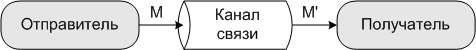
\includegraphics[width=.8\textwidth]{pict/basechannel} }
            \mode<article>{ 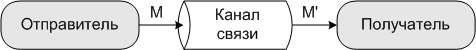
\includegraphics[width=.8\textwidth]{pict/basechannel} }
        \end{center}
        \caption{Базовая схема передачи информации}\label{pict:basechannel}
    \end{figure} 
    \mode<article>{См. рисунок \ref{pict:basechannel}}

    Можно выделить следующие виды \alert{каналов связи}:
    \begin{itemize}
        \item \alert{Секретный} гарантирует конфиденциальность, целостность и принадлежность M;
        \item \alert{Аутентичный} гарантирует только целостность и принадлежность M;
        \item \alert{Открытый} не гарантирует ничего в отношении M.
    \end{itemize}
\end{frame}


Криптографическая защита --- это защита на \emph{уровне представления} информации\footnote{Уровней доступа к информации, как известно, четыре: носителя, средств взаимодействия с носителем, \emph{представления}, содержания (смысла)}. Далее мы рассмотрим криптографические схемы, направленные на защиту конфиденциальности.

Конфиденциальность – это, как уже известно, недоступность третьим лицам. Первые два лица – это источник (отправитель) и получатель информации в процессе передачи информации. Третье лицо – злоумышленник, для которого передаваемая информация должна оставаться недоступной. Выход – ограничить доступ третьих лиц к каналу передачи информации, либо перекодировать информацию так, чтобы её восприятие стало им недоступно. Такое перекодирование называется шифрованием. Об особенностях шифрования и поговорим далее.

Разработкой методов шифрования (в том числе) занимается криптография. Исследованием творений криптографии на стойкость занимается криптоанализ. Оба направления, криптография и криптоанализ, объединяются в единую науку – криптологию.

Методы шифрования разделяют на два вида: симметричные и асимметричные. Очень важным условием для существования самой возможности шифрования является наличие \emph{секрета}.


\begin{frame}
    \frametitle{Схемы шифрования}
    \framesubtitle{Симметричная схема}
    \begin{figure}
        \begin{center}
            \mode<presentation>{ 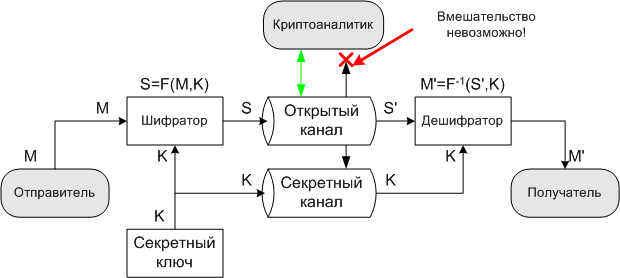
\includegraphics[width=.8\textwidth]{pict/symmcipher} }
            \mode<article>{ 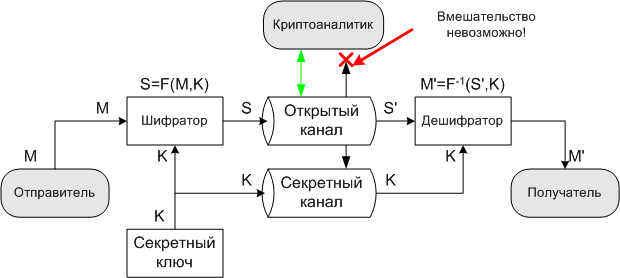
\includegraphics[width=.8\textwidth]{pict/symmcipher} }
        \end{center}
        \caption{Симметричная схема шифрования}\label{pict:symmcipher}
    \end{figure} 
    \mode<article>{См. рисунок \ref{pict:symmcipher}}
\end{frame}


Исходное сообщение (информация M) отправитель преобразует с помощью шифратора в шифротекст $S$. Для этого преобразования шифратором используется функция $F:M,K\rightarrow S$ , вторым аргументом которой является секретная информация – ключ $K$. Ключ $K$ известен только отправителю и получателю, они и только они  разделяют этот секрет. Злоумышленник, который в данной схеме назван криптоаналитиком, секретом $K$ овладеть не может \emph{по определению}! С выхода шифратора шифротекст $S$ передается через открытый канал получателю. При этом шифротекст может получить и криптоаналитик. Более того, криптоаналитик даже может внести изменения в шифротекст, и до получателя дойдет уже не $S$, а $S'$.  Получатель  восстанавливает из шифротекста $S'$ исходное сообщение $M'$ с помощью дешифратора. Дешифратором, используется функция $F^{-1}:S,K\rightarrow M$ , позволяющая выполнить обратное преобразование: $F^{-1}(F(M,K),K)=M$ . Без знания ключа восстановить из шифротекста $S$ исходное сообщение $M$ практически невозможно. Даже зная функции $F$  и $F^{-1}$ , криптоаналитик, не зная ключа $K$, не в силах восстановить сообщение. В этом, к слову, и заключается важнейшее правило криптографии, сформулированное голландским криптологом Керкхоффом: стойкость шифра должна зависеть только от секретности ключа.

Криптоаналитик может испортить жизнь законным участникам обмена, исказив или подменив шифротекст. Увы, осмысленных изменений без знания ключа ему не сделать! Более того, если до шифрования в сообщение $M$ была внесена избыточность с целью защиты целостности, то факт вмешательства будет обнаружен получателем после дешифрования и заработает стратегия повторной передачи.

Следует обратить внимание, что в схеме используется \emph{секретный канал}. Спрашивается, раз есть секретный канал для передачи ключей, то почему же не использовать это сокровище для передачи сообщений? Увы, секретный канал слишком дорог. Использовав его один раз для обмена секретным ключом, законные отправитель и получатель теперь могут организовать секретный канал передачи на основе любого открытого, что гораздо дешевле.

\emph{Симметричным} шифр назван потому, что один и тот же ключ применяется как для шифрования, так и для дешифрования.
Существует множество симметричных шифров. Современный симметричный шифр стоек и математически обоснован. Стандартом в настоящее время является шифр AES, в девичестве Rijndael. Активно используется и модификация бывшего стандарта DES --- шифр DES3. Впрочем, помимо стандартов существует множество проверенных временем шифров, которые могут использоваться в системах защиты информации. Использовать недавно созданный \emph{гениальным} автором \emph{сверхстойкий} шифр нужно лишь в целях информационного самоубийства.


\begin{frame}
    \frametitle{Достоинства и недостатки}
    
    \begin{itemize}
        \item Секретный ключ должны знать оба абонента.
        \item Для того, чтобы организовать безопасный обмен между $n$ абонентами требуется распределить 
        \[\binom{n}{2}=\frac{n(n-1)}{2}\]
        ключей, что при большом $n$ становится весьма затруднительно. Для решения задачи распределения симметричных ключей обычно прибегают к схемам с \alert{доверенным} лицом.
        \item На практике симметричные шифры работают на порядки быстрее асимметричных.
    \end{itemize}
\end{frame}


\begin{frame}
    \frametitle{Схемы шифрования}
    \framesubtitle{Ассиметричная схема}
    \begin{figure}
        \begin{center}
            \mode<presentation>{ 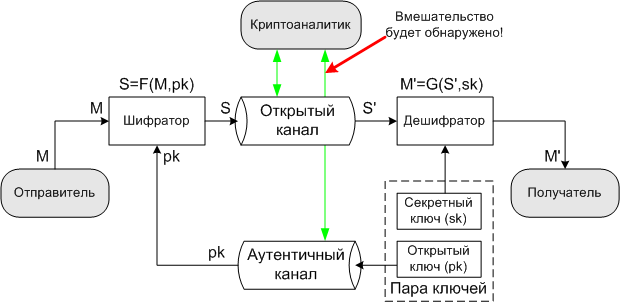
\includegraphics[width=.8\textwidth]{pict/asymmcipher} }
            \mode<article>{ 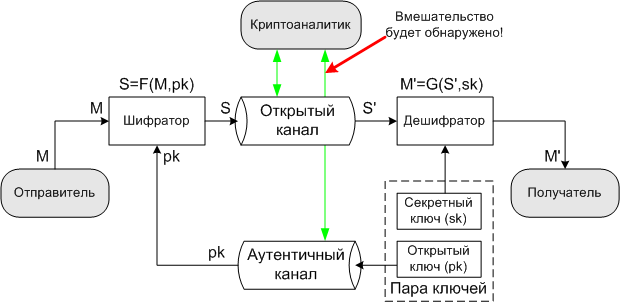
\includegraphics[width=.8\textwidth]{pict/asymmcipher} }
        \end{center}
        \caption{Асимметричная схема шифрования}\label{pict:asymmcipher}
    \end{figure} 
    \mode<article>{См. рисунок \ref{pict:asymmcipher}}
\end{frame}


Особенность ассиметричного шифра заключается в том, что для шифрования и дешифрования используются разные ключи $(sk, pk)$. Пара ключей $\langle sk, pk\rangle$ генерируется получателем относительно легко. Один из этой пары ключей будет открытым $pk$ (public key), и может быть передан неограниченному числу отправителей. Ключ $sk$, парный открытому, держится отправителем в секрете: $sk$ – secret(private) key. Важнейшей особенностью схемы является то, что, зная открытый ключ $pk$, вычислить по нему секретный $sk$ практически невозможно. Шифрование осуществляется с помощью открытого ключа, дешифрование с помощью секретного. Более того, восстановить из шифротекста исходное сообщение без знания секретного ключа практически невозможно: $G(F(M, pk), sk)=M$. Криптоаналитик может завладеть открытым ключом (впрочем великодушный получатель может сразу послать ему копию), но дешифровать сообщения он не сможет. Ему остается только слать получателю зашифрованные проклятия. Расшифровать сообщения может только обладатель секрета $sk$.

Шифруют все, расшифровывает один.

Внимательный читатель обратил внимание на то, что открытый ключ $pk$ передается по аутентичному каналу. Да, открытый канал для передачи открытого ключа $pk$ нельзя использовать ни в коем случае! Представте себе, что злоумышленник сгенерировал свою пару $\langle sk1, pk1\rangle$, перехватил $pk$, когда он передавался отправителю, и вместо перехваченного ключа послал отправителю от имени получателя свой открытый ключ $pk1$. Отправитель, будучи уверен в том, что $pk1$ – это открытый ключ получателя, зашифрует для него сообщение. Злоумышленник перехватит его, расшифрует на своем $sk1$, внесет необходимые поправки, зашифрует перехваченным $pk$ и отошлет получателю. Отправитель и получатель отныне общаются через двуликого Януса. Как же быть? Нужно использовать \alert{аутентичный} канал. Аутентичный канал гарантирует целостность и принадлежность информации. Получив данные по такому каналу, вы уверены в том, что информация в процессе передачи не была испорчена (целостность), и в том, что вы получили её именно от того, от кого и рассчитывали получить (принадлежность). Аутентичный канал дороже открытого, но дешевле секретного. Можно использовать секретный канал вместо аутентичного, хуже не будет, а в ряде случаев это просто необходимо.

Распространенные и проверенные временем схемы ассиметричного шифрования: RSA (факторизация), Диффи-Хеллмана (дискретное логарифимирование), алгоритмы на основе эллиптических кривых ECES.


\begin{frame}
    \frametitle{Достоинства и недостатки}
    
    \begin{itemize}
        \item Публичный (открытый) ключ должен распространяться по аутентичным каналам\footnote{Когда злоумышленник в состоянии перехватить открытый ключ абонента $A$ и подменить его собственным открытым, он может контролировать (в том числе и модифицировать) сообщения $A$}.
        \item Для того, чтобы организовать безопасный обмен между $n$ абонентами требуется распределить всего $n$ ключевых пар\footnote{При этом нет необходимости прибегать к услугам доверенных лиц}.
        \item На практике асимметричные шифры работают на порядки медленнее симметричных.
    \end{itemize}
\end{frame}


Т.к. асимметричные алгоритмы работают медленно, то применяются комбирированные схемы: нагрузка шифруется на случайно сгенерированном сеансовом ключе, который затем шифруется по асимметричной схеме.
\begin{frame}
    \frametitle{Схемы шифрования}
    \framesubtitle{Комбинированная схема}
    \begin{figure}
        \begin{center}
            \mode<presentation>{ 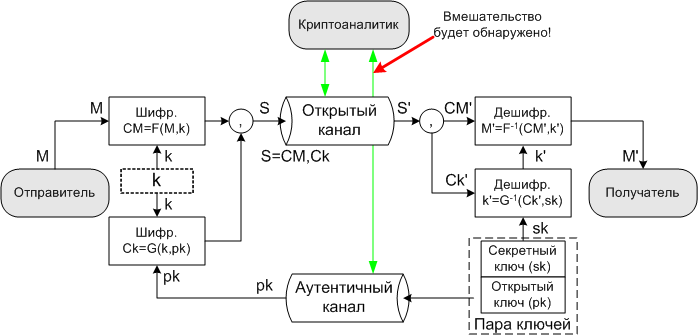
\includegraphics[width=.8\textwidth]{pict/combocipher} }
            \mode<article>{ 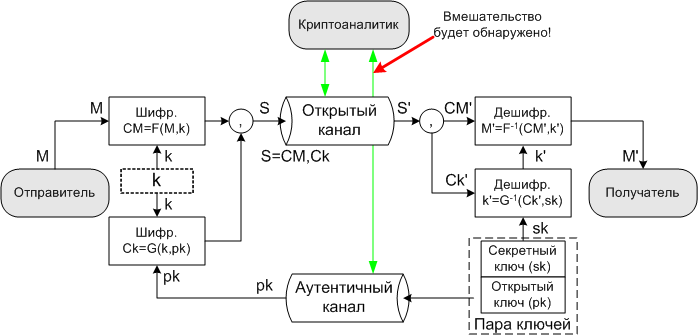
\includegraphics[width=.8\textwidth]{pict/combocipher} }
        \end{center}
        \caption{Комбинированная схема шифрования}\label{pict:combocipher}
    \end{figure} 
    \mode<article>{См. рисунок \ref{pict:combocipher}}
\end{frame}



\begin{frame}
    \frametitle{Абсолютно стойкий и вычислительно стойкий шифр}
    
    \alert{Абсолютно стойкий (идеальный)} шифр --- шифр для которого задача подбора ключа для шифротекста эквивалентна угадыванию открытого текста.
    
    Условие выполнимо, например, если длина ключа $K$ равна длине сообщения $M$:
    \begin{itemize}
        \item Шифрование: \(S=M\oplus K.\)
        \item Расшифрование: \(M=S\oplus K=M\oplus K\oplus K=M\oplus 0.\)
    \end{itemize}
    Причем ключ случаен и используется единожды. Практическим примером абсолютно стойкого шифра является \alert{шифровальный блокнот Вернама}.
    
    Стойкость \alert{практически стойких} или \alert{вычислительно стойких} шифров определяется вычислительными возможностями криптоаналитика.
\end{frame}


Напоследок следует сказать несколько слов об идеальном шифре. Точнее об идеально стойком шифре. Существует ли такой? Существует! Это шифровальный блокнот Вернама. Шифр симметричный. Как им пользоваться? В обстановке строгой секретности изготавливается два идентичных блокнота. На каждом листке такого блокнота напечатана одна буква (можно распечатать в блокноте, например, выбранный наугад абзац из любимой книжки или случайные буквы). Первая буква сообщения «складывается» с буквой на первой страничке блокнота. На самом деле, конечно, складываются порядковые номера букв в алфавите, и от полученной суммы находится остаток от деления на общее количество букв в алфавите. Это и будет номер буквы шифротекста. А+А=А (номера с нуля!), Б+Б=В, В+Г=Е, Я+А=Я, Я+Б=А… Первую букву шифротекста выписываем на бумажку, а первую страничку блокнота съедаем. И так далее. В процессе дешифрования в том же порядке съедается и второй блокнот. При этом буквы со страниц блокнота <<вычитаются>> из шифротекста. Аналогом шифра Вернама в двоичных вычислительных машинах будет сложение битового представления текста $M$ с битовым представлением ключа $K$ по <<модулю два>>: $S=M\oplus K$ . Дешифрование заключается в сложении шифротекста $S$ с ключом $K$: $S\oplus K=M\oplus K\oplus K=M\oplus 0=M$ . Ключ должен быть уничтожен. В обоих случаях видно, что длина ключа равна длине сообщения. И очевидно, что вместо того, чтобы подбирать ключ, криптоаналитику лучше сесть и сочинить свое сообщение подходящей длины. На том и успокоиться.


\subsection{Организация аутентичных каналов}


Как можно доверять тому, что открытый ключ $pk_A$ принадлежит именно $A$, а не другому лицу? Гарантии тому дает использование аутентичного канала в ассиметричной схеме. Но как создать подобный канал? Один из способов --- использовать сертификаты.

Далее рассмотрим аутентификацию, использующую сертификаты, для чего вначале обсудим схему цифровой подписи (ЭЦП) дающую гарантии целостности и принадлежности подписанной информации.

Кстати, федеральным законом об электронной  цифровой подписи, принятом в 2002 году, установлен юридический статус этому понятию. Цифровая подпись является доказательством в суде, как и рукописная подпись под бумажным документом. 


\begin{frame}
    \frametitle{Цифровая подпись}
    \begin{figure}
        \begin{center}
            \mode<presentation>{ 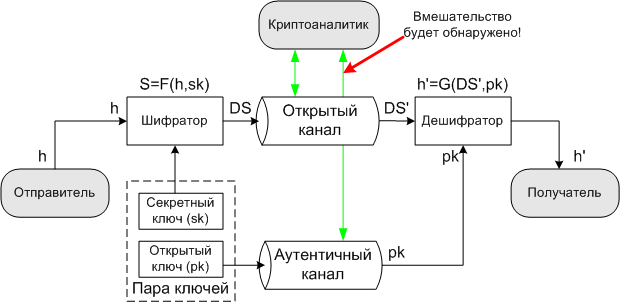
\includegraphics[width=.8\textwidth]{pict/signature} }
            \mode<article>{ 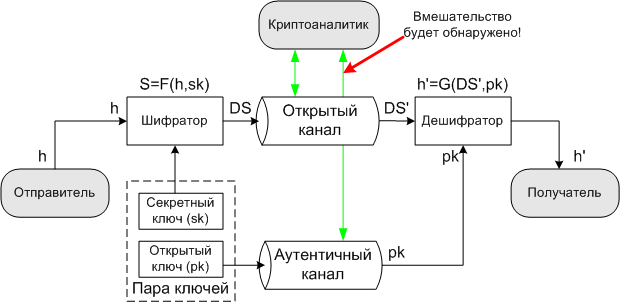
\includegraphics[width=.8\textwidth]{pict/signature} }
        \end{center}
        \caption{Цифровая подпись}\label{pict:signature}
    \end{figure} 
    \mode<article>{См. рисунок \ref{pict:asymmcipher}}
\end{frame}

Как видно, схема очень похожа на схему ассиметричного шифрования. Все сказанное в отношении схемы шифрования справедливо и для цифровой подписи, за исключением того, что обладателем секрета теперь является отправитель, и шифрование слепка сообщения $h$ производится на секретном ключе $sk$. Цифровой подписью называется результат шифрования слепка – $DS$. Без знания секретного ключа $sk$ шифрование невозможно. Любой желающий, имеющий открытый ключ $pk$, может дешифровать сообщение (проверить подпись).

Итак, зашифровать слепок может только один отправитель, а расшифровать --- любой желающий проверить подпись получатель.

При этом получатель, расшифровывающий $DS$ открытым ключом $pk$, уверен в том, что зашифровать слепок мог только обладатель секретного ключа $sk$ (парного открытому ключу $pk$). Уверен потому, что получил открытый ключ по аутентичному каналу.

Впрочем, пока не ясно, что представляет собой слепок $h$ сообщения $M$. Слепок может представлять собой копию сообщения $M$. Обычно и сообщение $M$, и его цифровая подпись DS передаются одним блоком $\langle M,DS\rangle$. Получателю достаточно расшифровать цифровую подпись $DS$ и сравнить с $M$. Совпадение будет означать, что полученное $M$ аутентично, так как гарантированы его целостность и принадлежность отправителю. Злоумышленник не сможет внести идентичные изменения в сообщение и в подпись, так как должен для этого вновь зашифровать измененную копию $M$, а это вычислительно невозможно без обладания секретным ключом $sk$. На практике (в целях экономии памяти) слепок $h$ формируется как результат хеширования сообщения с помощью криптографической хеш-функции: $h=H(M)$. Аналогично, сообщение $M$ и его цифровая подпись $DS=F(H(M), sk)$ передаются одним блоком $\langle M,DS\rangle$. Получатель, разделив, блок на части $M'$ и $DS'$, находит $H(M')$ и сравнивает с расшифрованной подписью $h'=G(DS', pk)$. Если эти величины равны --- сообщение $M$ аутентично. Злоумышленник, подделывая подпись, столкнется с необходимостью, либо зашифровать вычисленный им слепок $H(M')$ измененного сообщения $M'$ (что вычислительно невозможно без знания $sk$), либо подобрать такое осмысленное сообщение $M'$, чтобы оно давало такой же хеш, что и исходное $M$ (что вычислительно невозможно, так как $H$ обладает стойкостью к коллизиям первого рода).

Подписанному сообщению можно доверять в том случае, если вы доверяете подписавшему. Для того, чтобы быть уверенным в том, что открытый ключ ассиметричной схемы принадлежит пользователю $A$, нужно, чтобы доверенное лицо подписало блок данных $A, pk_A$. Такой подписанный блок называется цифровым сертификатом открытого ключа. Сертифицированный открытый ключ становится <<аутентичным>>.

%QUEST: что такое аутентичный открытый ключ?

\begin{frame}
    \frametitle{Криптографическая аутентификация}
    \framesubtitle{Сертификаты, цифровая подпись}
    Согласно стандарту X.509 сертификат открытого ключа пользователя $A$ --- $cert_A$, содержит значения следующих параметров.
    \begin{enumerate}
        \item Уникальное имя пользователя $A$.
        \item Открытый ключ $A$: $pk_A$.
        \item Назначение ключа $pk_A$ (для шифрования или для проверки ЭЦП).
        \item Период действия сертификата (даты начала и конца периода)
        \item Серийный номер сертификата.
        \item Уникальное имя доверенного лица, подписавшего сертификат.
        \item Идентификатор и параметры алгоритма ЭЦП, которым подписан $cert_A$.
    \end{enumerate}
\end{frame}

Из рассмотренных ассиметричных схем видно, что открытые (и соответственно закрытые) ключи могут использоватся двояко: для шифрования и для дешифрования! Использовать открытый ключ, предназначенный для проверки ЭЦП для шифрования использовать нельзя!


\begin{frame}
    \frametitle{Криптографическая аутентификация}
    \framesubtitle{Пример сертификата}
    \begin{figure}
        \begin{center}
            \mode<presentation>{ 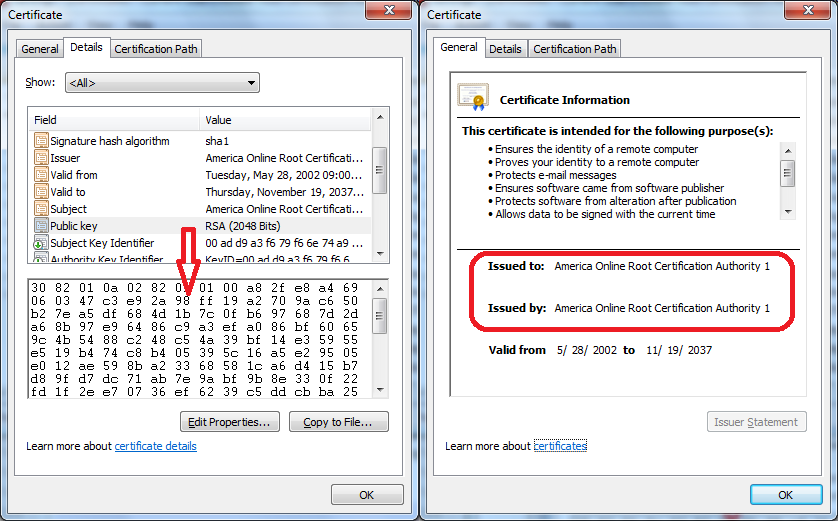
\includegraphics[width=.74\textwidth]{pict/certscreen} }
            \mode<article>{ 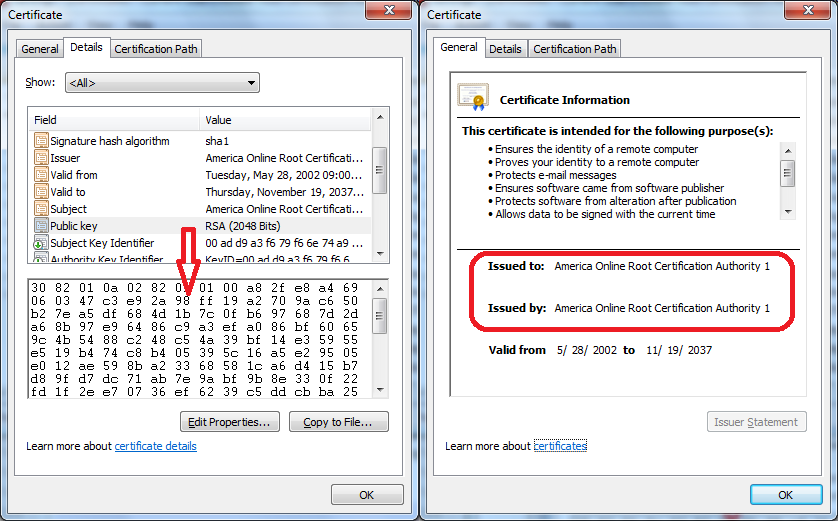
\includegraphics[width=.74\textwidth]{pict/certscreen} }
        \end{center}
        \caption{Пример сертификата}\label{pict:certscreen}
    \end{figure}
    \mode<article>{См. рисунок \ref{pict:certscreen}}
\end{frame}


В операционной системе обычно содержатся заранее установленные производителем сертификаты доверенных лиц, которым пользователь доверяет хотя бы в силу того, что приобрел данную ОС. О моделях построения центров сертификации (т.е. способов проверки подлинности сертификатов) поговорим на следующих лекциях.


\section{Симметричные схемы}


\begin{frame}
    \frametitle{Блок Фейстеля (Файстеля)}
    
    \begin{figure}
        \begin{center}
            \mode<presentation>{ 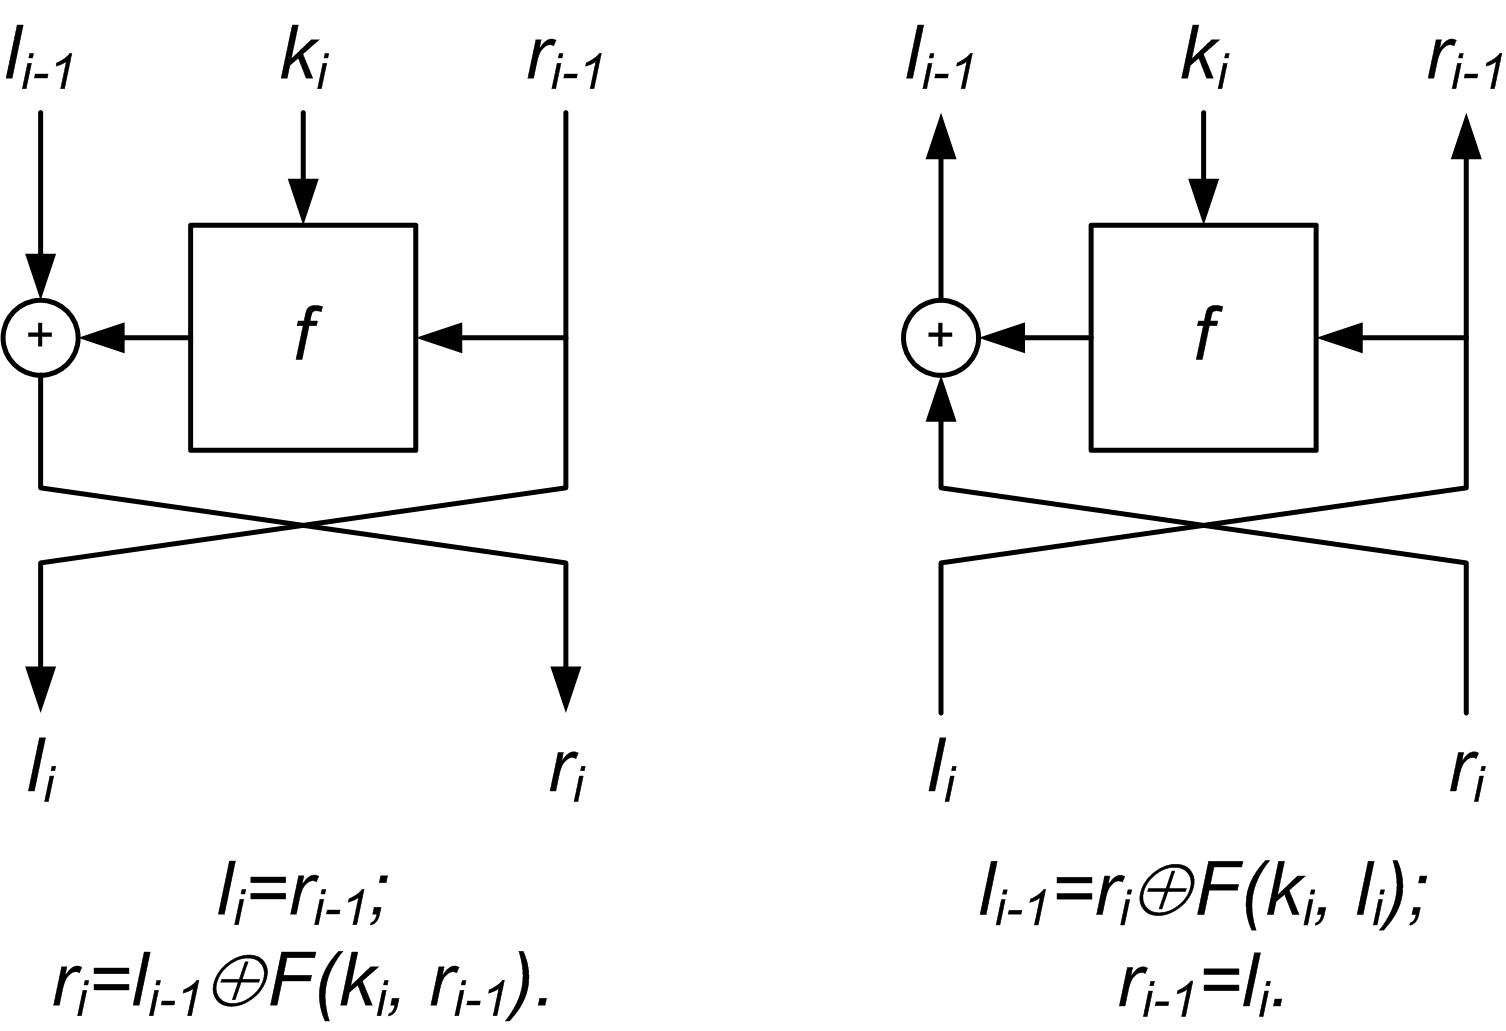
\includegraphics[width=.74\textwidth]{pict/feistelh} }
            \mode<article>{ 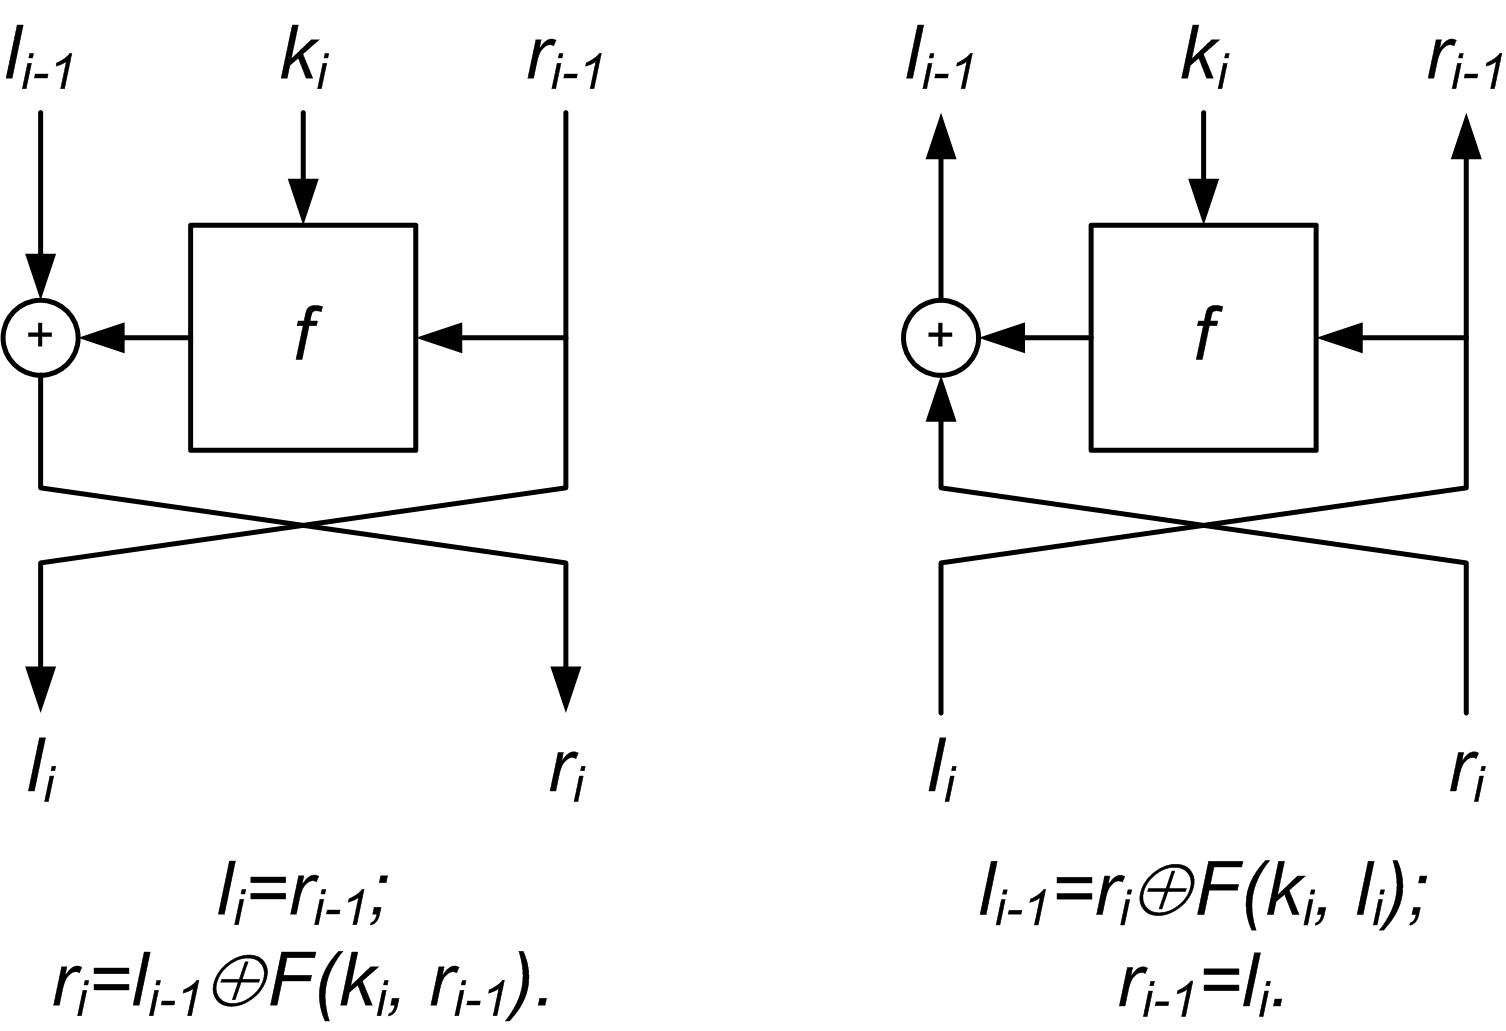
\includegraphics[width=.74\textwidth]{pict/feistelh} }
        \end{center}
        \caption{Блок Фейстеля}\label{pict:feistelh}
    \end{figure}
    \mode<article>{См. рисунок \ref{pict:feistelh}}
\end{frame}


\begin{frame}
    \frametitle{Раунды из блоков Фейстеля}
    
    \begin{figure}
        \begin{center}
            \mode<presentation>{ 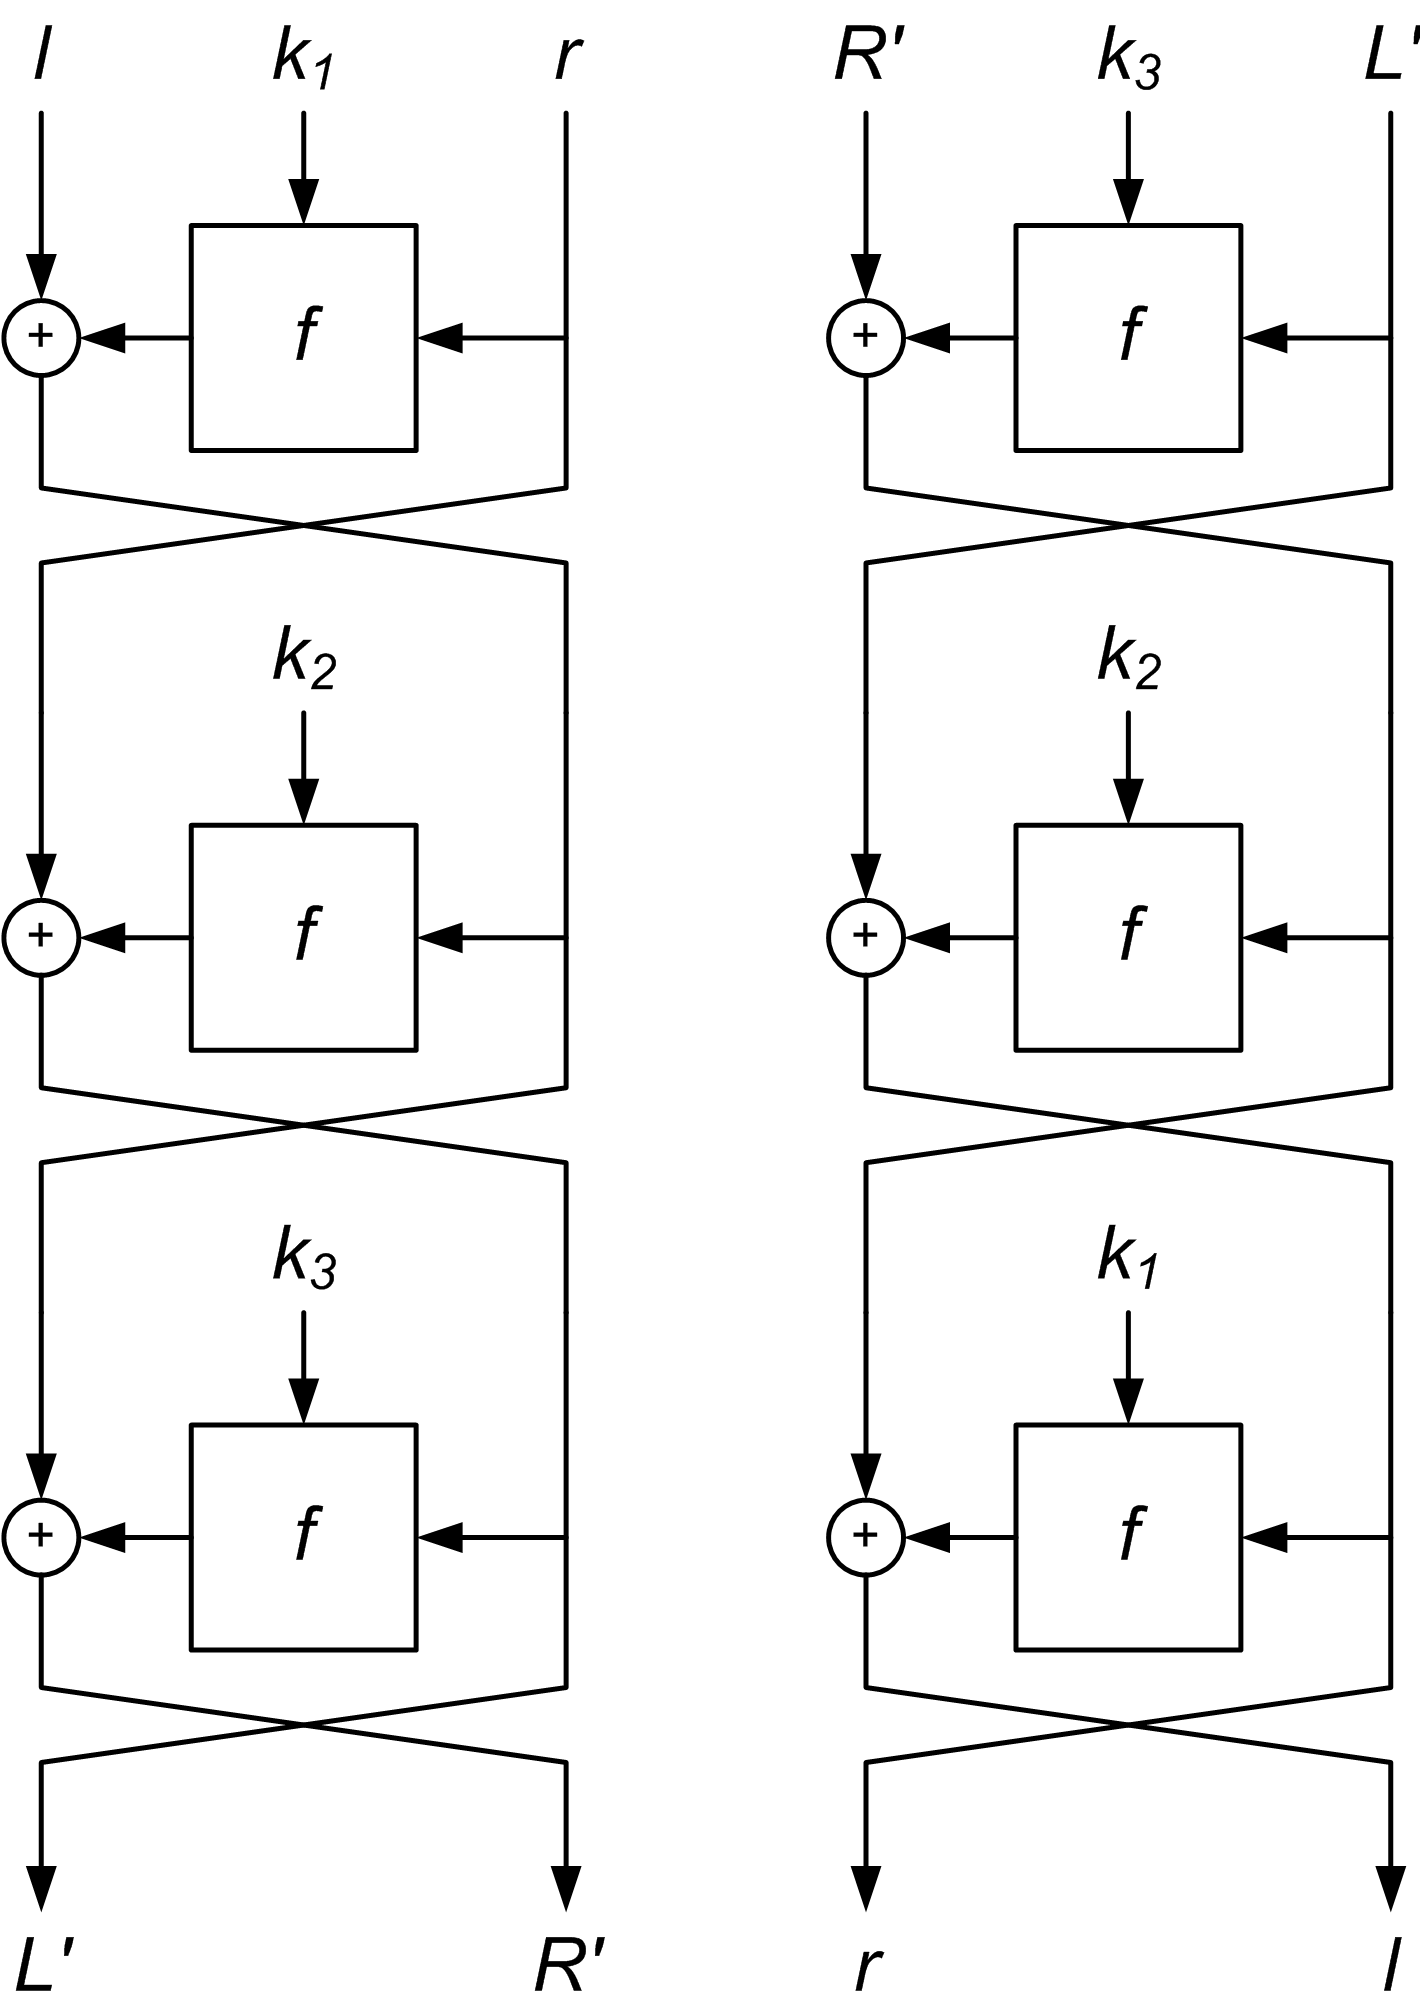
\includegraphics[height=.74\textheight]{pict/feistelhrounds} }
            \mode<article>{ 
                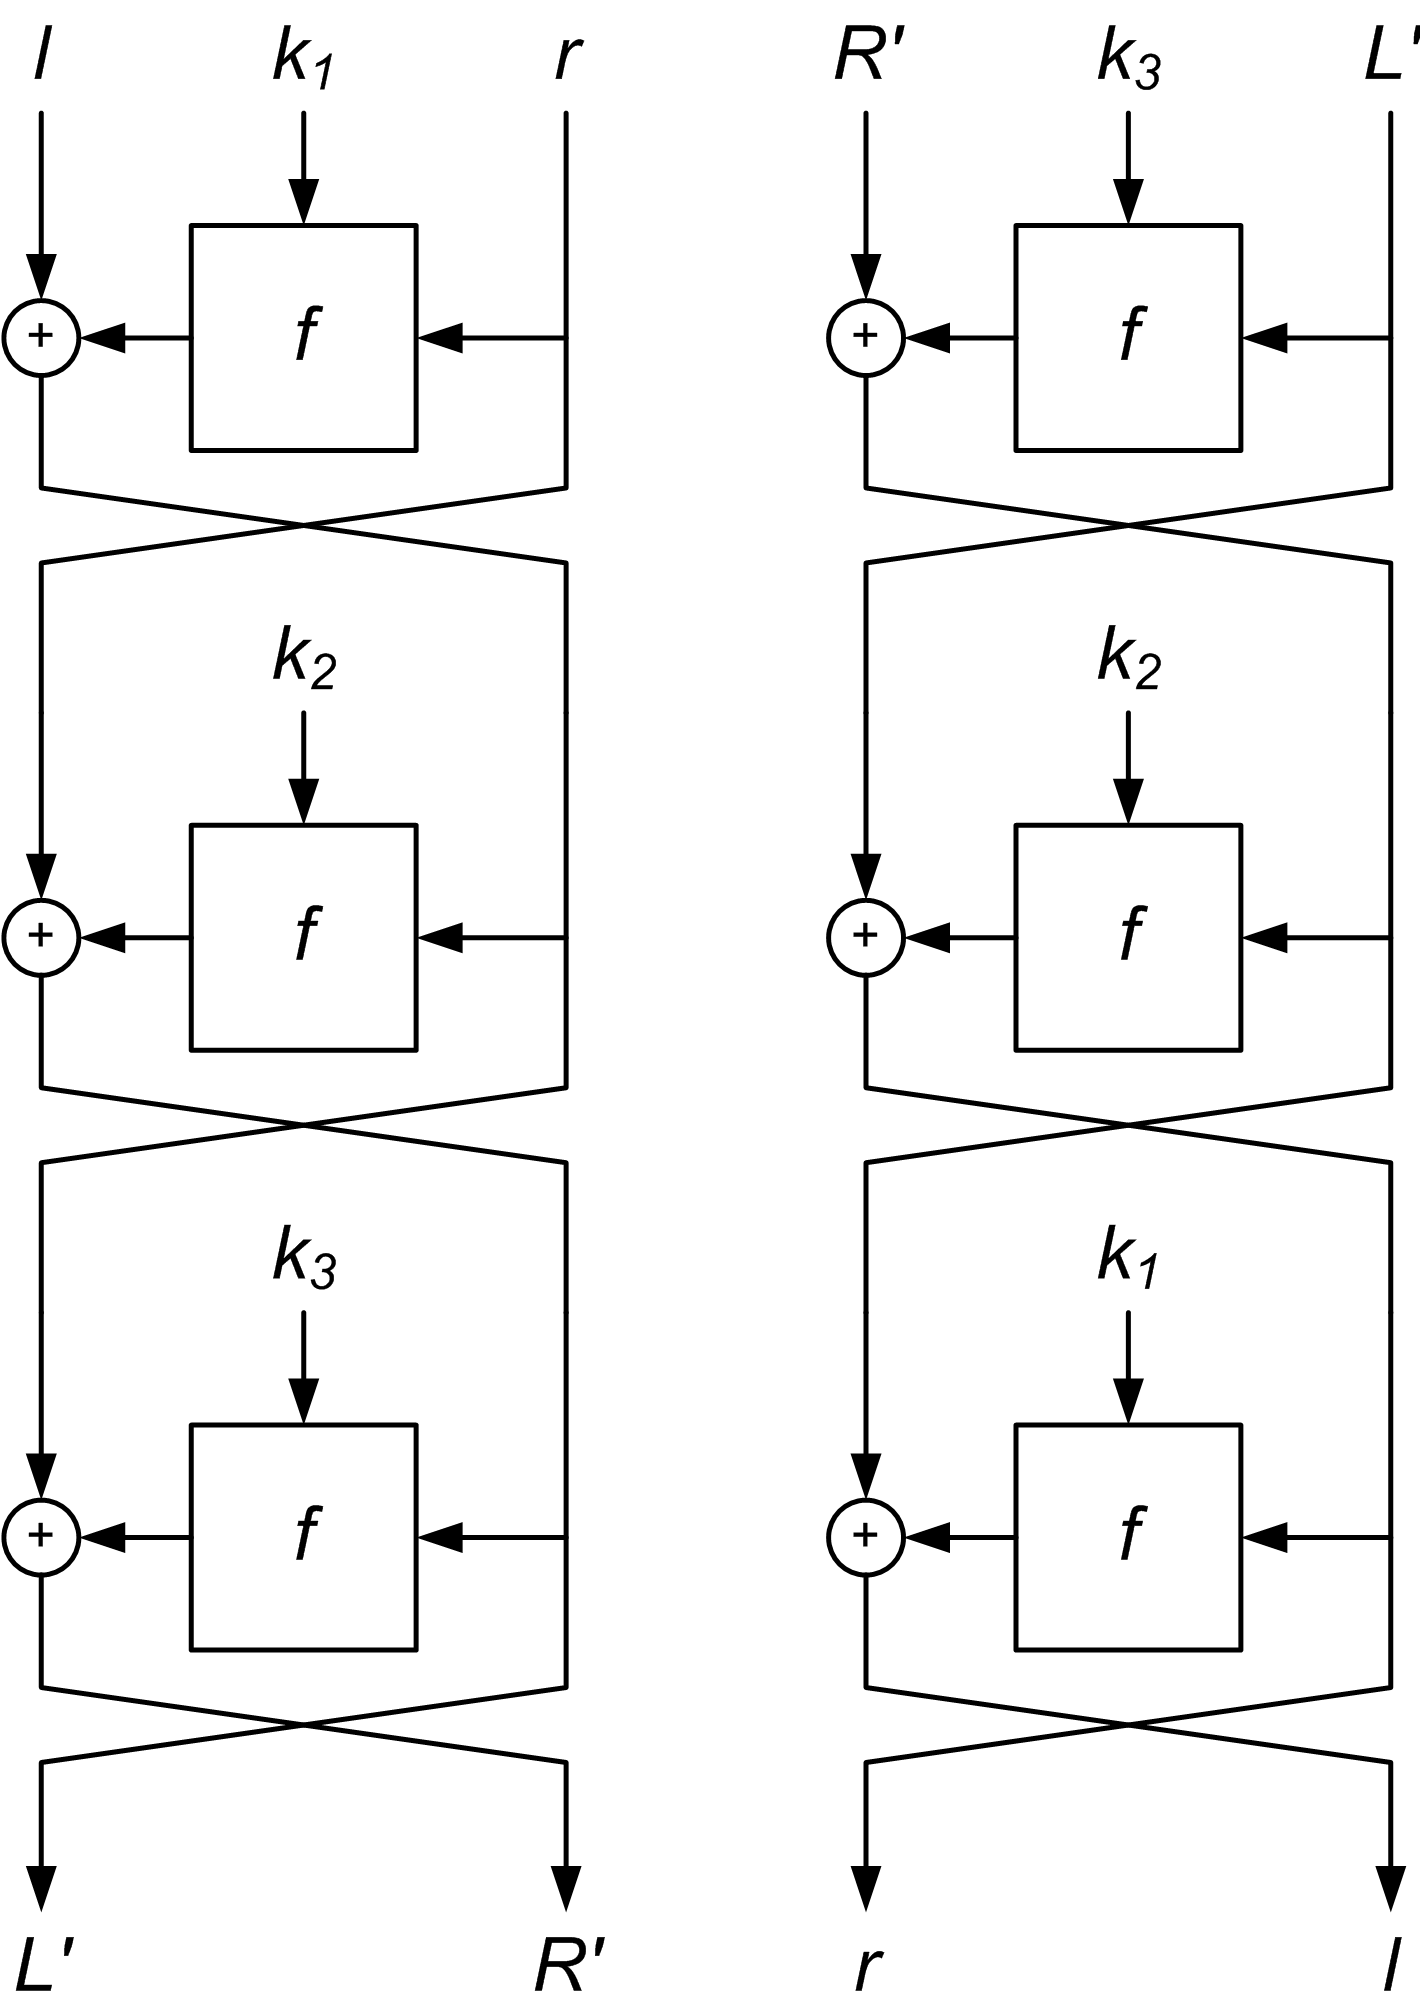
\includegraphics[width=.74\textwidth]{pict/feistelhrounds} 
                \caption{Раунды из блоков Фейстеля}\label{pict:feistelhrounds}
            }
        \end{center}
    \end{figure}
    \mode<article>{См. рисунок \ref{pict:feistelhrounds}}
\end{frame}

Одна и та же аппаратная реализация для шифрования и для обратного процесса. Смените порядок ключей. И лево смените направо.


\subsection{ГОСТ 28147-89}


\begin{frame}
    \frametitle{ГОСТ 28147-89}
    
    Отечественный стандарт шифрования данных.
    
    Размер ключа составляет 256 бит, а размер блоков 64 бит.
\end{frame}


\begin{frame}
    \frametitle{Блок Фейстеля для ГОСТ 28147-89}
    
    \begin{figure}
        \begin{center}
            \mode<presentation>{ 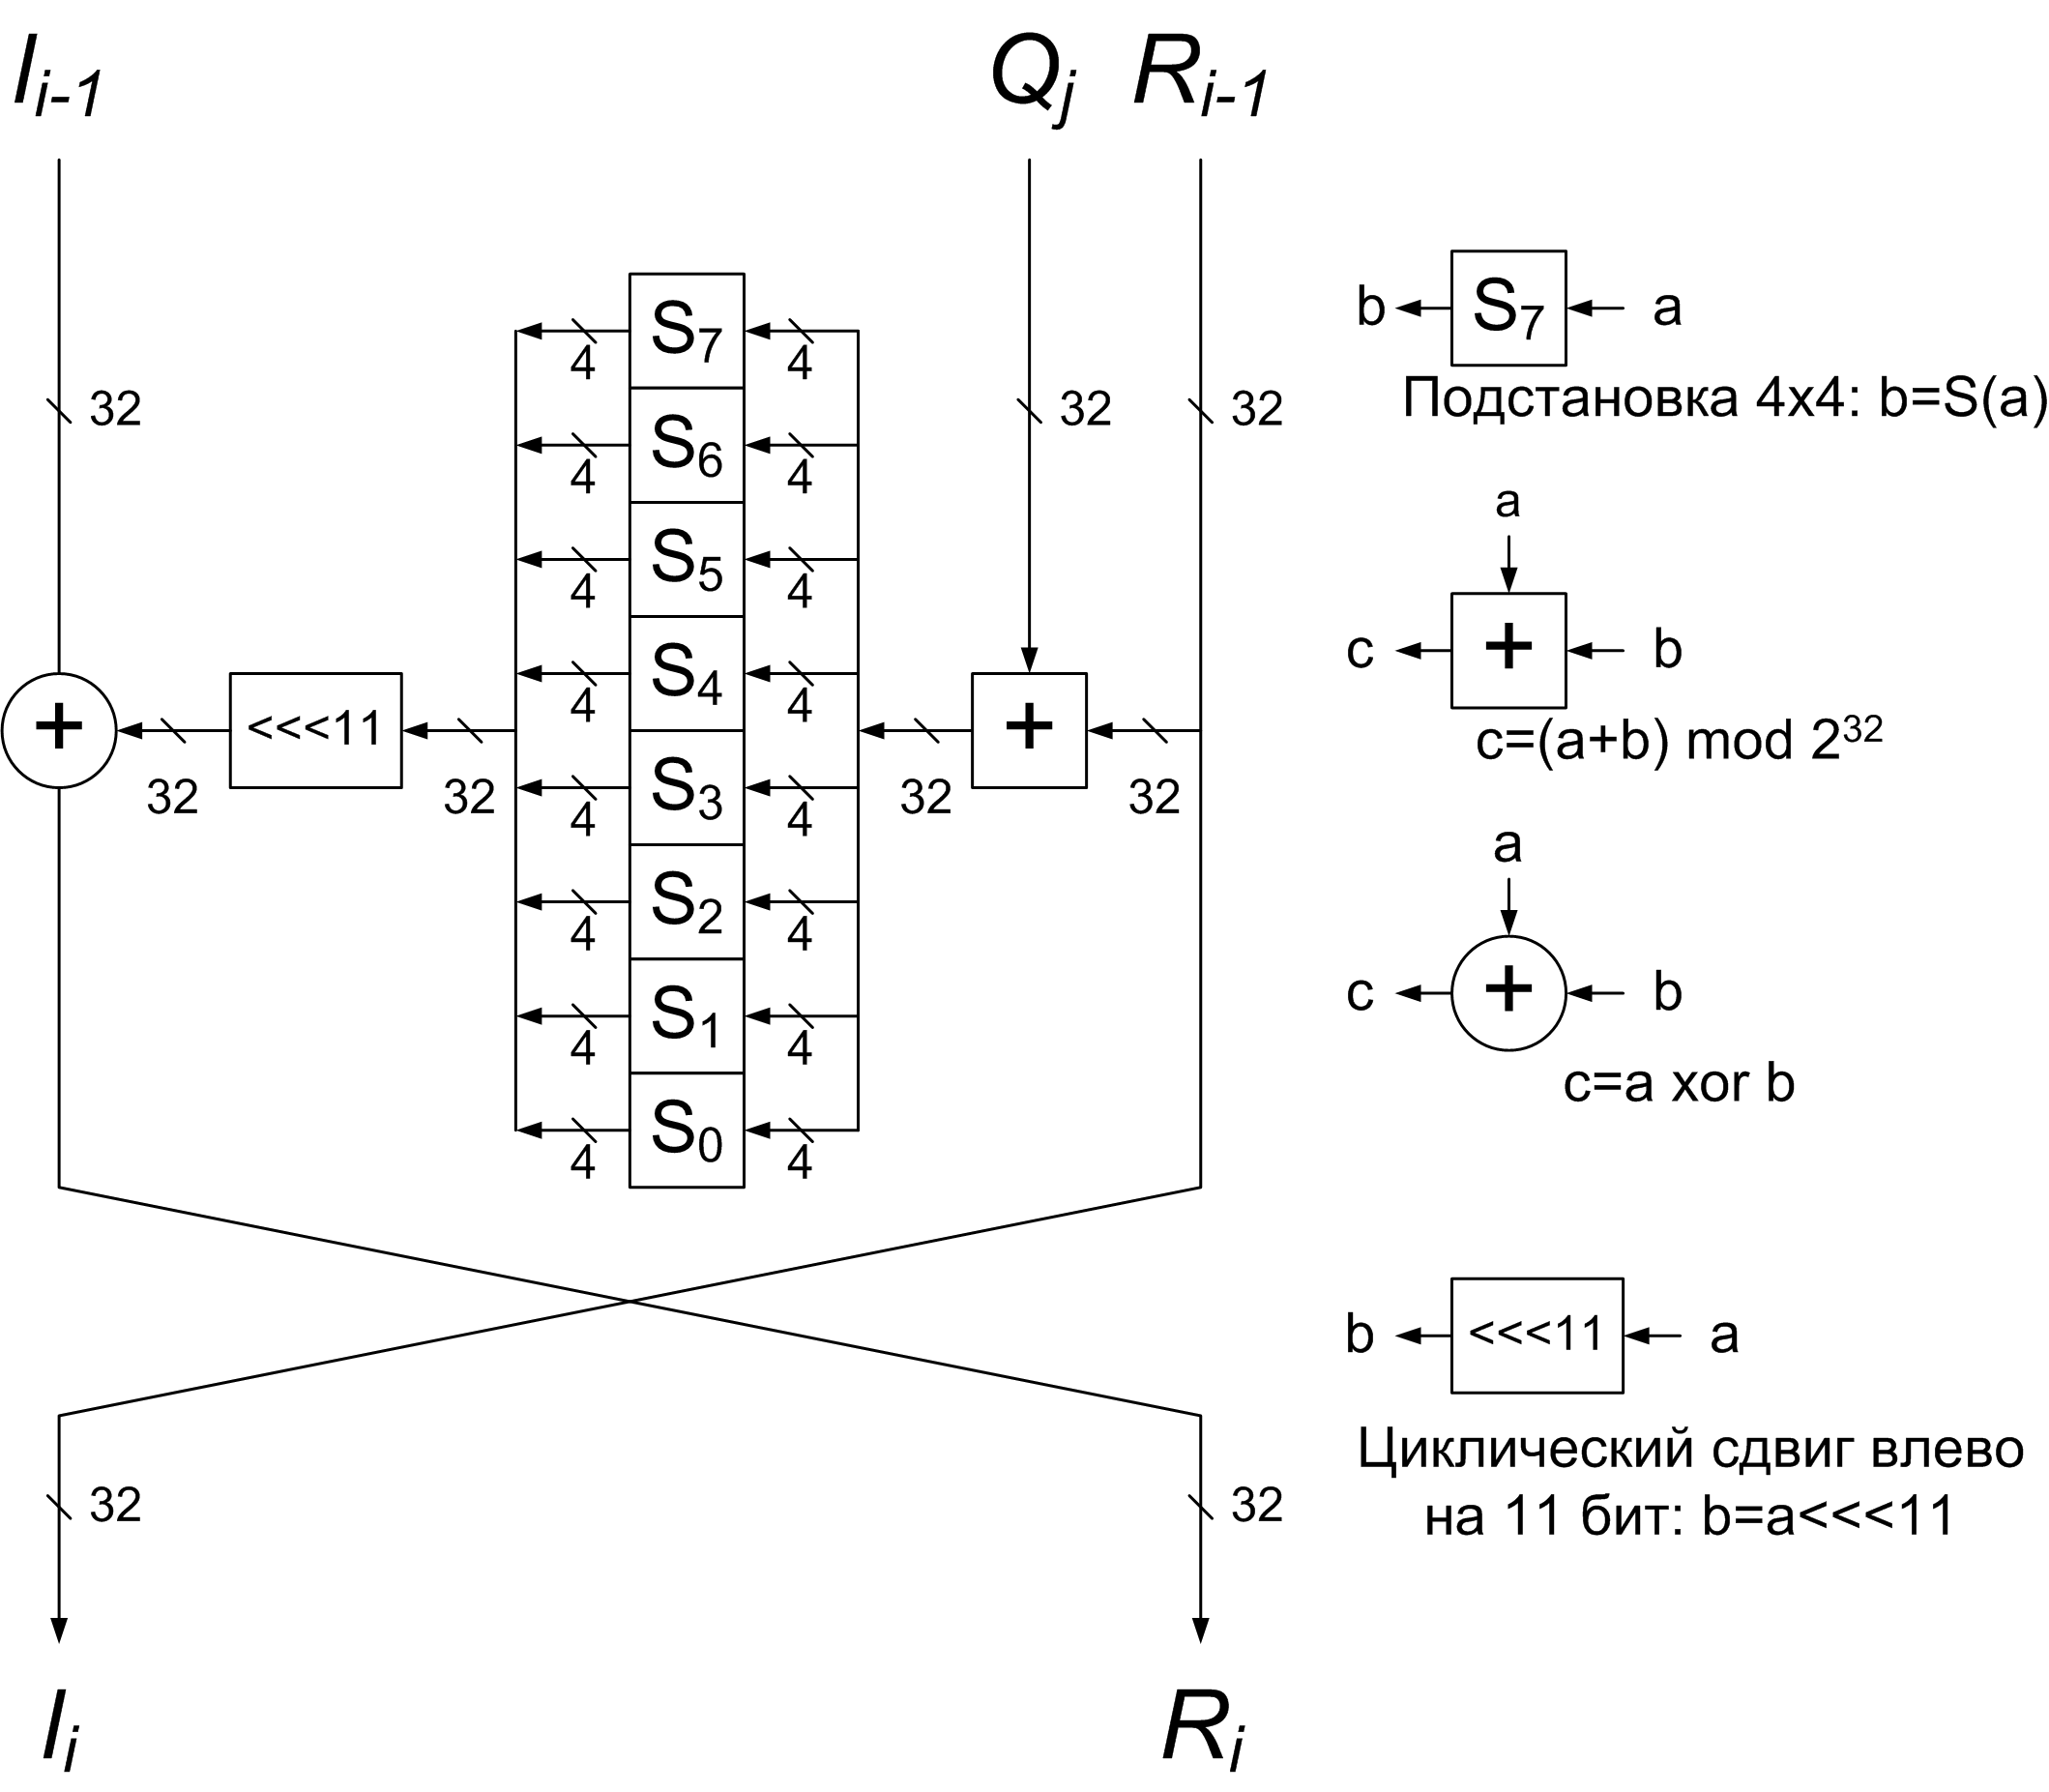
\includegraphics[height=.74\textheight]{pict/gost} }
            \mode<article>{ 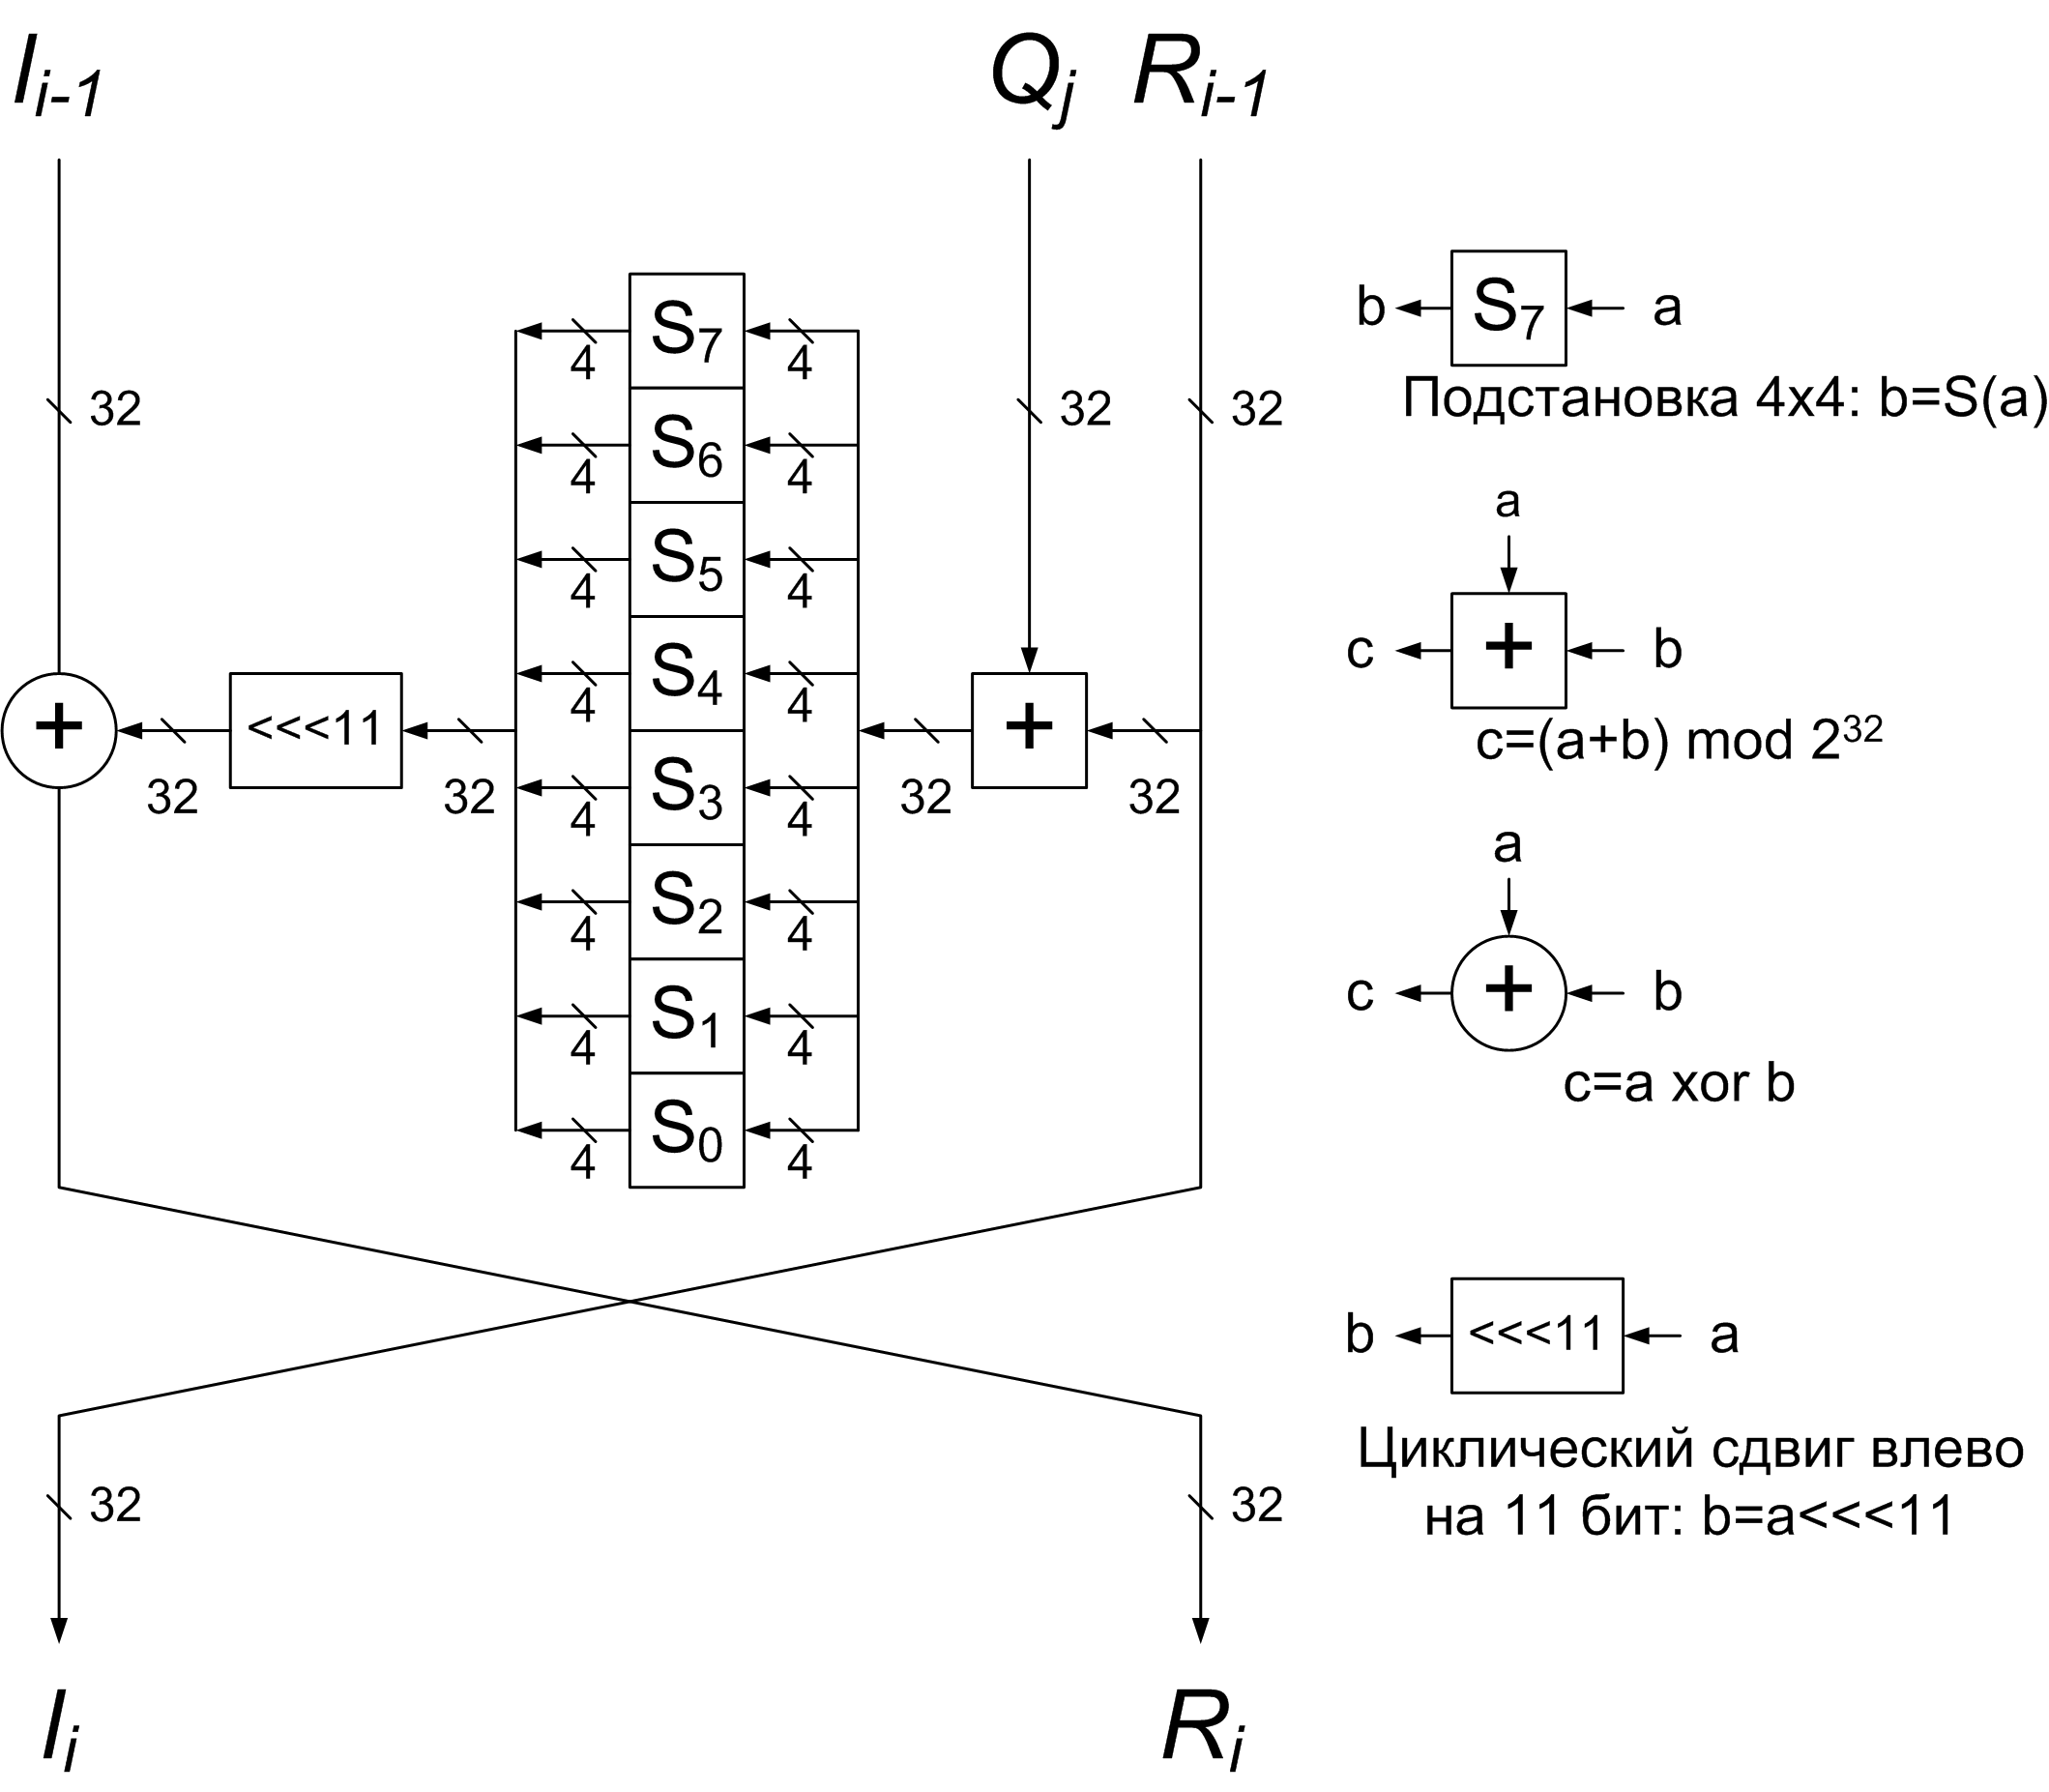
\includegraphics[width=.74\textwidth]{pict/gost} }
        \end{center}
        \caption{Блок Фейстеля для ГОСТ 28147-89}\label{pict:gost}
    \end{figure}
    \mode<article>{См. рисунок \ref{pict:gost}}
\end{frame}


\begin{frame}
    \frametitle{Шифрование по ГОСТ 28147-89}
    
    На входе 64 битный блок $T$ – конкатенация двух 32 битных подблоков $L$ и $R$: $T=L|R$
    \begin{enumerate}
        \item Установить счетчик $i=1$.
        \item \label{enr:gostEncRound} Присвоить значение подблока $R$ переменной $V$: $V=R$.
        \item Вычислить номер $j$ выбираемого подключа: $j = (i<25) ? ((i-1) \mod 8) : ((32-i) \mod 8)$.
        \item Преобразовать подблок $R$: 
            $R=(R+Q_j) \mod 2^{32}$,
            $R=S_7(r_7)|S_6(r_6)|S_5(r_5)|S_4(r_4)|S_3(r_3)|S_2(r_2)|S_1(r_1)|S_0(r_0)$, при 
            $R= r_7|r_6|r_5|r_4|r_3|r_2|r_1|r_0$,
            $R=R<<<11$,
            $R=R \oplus L$.
        \item Преобразовать подблок $L$: $L=V$.
        \item Если $i<32$, то $i=i+1$ и к шагу \ref{enr:gostEncRound}.
        \item Стоп.
    \end{enumerate}
    На выходе: 64 битный $C=L|R$.
\end{frame}


\begin{frame}
    \frametitle{Расшифрование по ГОСТ 28147-89}

    На входе 64 битный блок $C$ --- конкатенация двух 32 битных подблоков $L$ и $R$: $C=L|R$.
    \begin{enumerate}
        \item Установить счетчик $i=1$.
        \item \label{enr:gostDecRound} Присвоить значение подблока $L$ переменной $V$: $V=L$.
        \item Вычислить номер выбираемого подключа: 
            $j = (i<9) ? ((i-1) \mod 8) : ((32-i) \mod 8)$
        \item Преобразовать подблок $L$: 
            $L=(L+Q_j) \mod 2^{32}$,
            $L=S_7(l_7)|S_6(l_6)|S_5(l_5)|S_4(l_4)|S_3(l_3)|S_2(l_2)|S_1(l_1)|S_0(l_0)$, при 
            $L=l_7|l_6|l_5|l_4|l_3|l_2|l_1|l_0$,
            $L=L<<<11$,
            $L=L \oplus L$.
        \item Преобразовать подблок $R$: $R=V$
        \item Если $i<32$ то $i=i+1$ и к шагу \ref{enr:gostDecRound}.
        \item Стоп.
    \end{enumerate}
    На выходе: 64 битный $T=L|R$.
\end{frame}


\subsection{DES, DES3}


\begin{frame}
    \frametitle{DES, DES3}
    
    DES --- Data Encryption Standard. Опубликован NIST в январе 1977 года.
    
    Размер ключа составляет 56 бит, а размер блоков 64 бит. 
    
    DES морально устарел (в первую очередь из за небольшой длины ключа), в настоящее время продолжает использоваться его модификация DES3, позволяющая увелечить длину ключа до $3\times 56=168$ бит
\end{frame}


64 битный открытый текст подвергается начальной перестановке $P$ и проходит 16 раундов преобразований Фейстеля. В каждом раунде используется 48 битный подключ, генерируемый для каждого раунда отдельно на основе 56 битного ключа. Получившийся в виде двух половинок $L_16$ и $R_16$ результат поступает на блок перестановки $P^{-1}$, обратной начальной см. рис. \ref{}. %TODO

\begin{frame}
    \frametitle{Раунды Фейстеля для DES}

    \begin{figure}
        \begin{center}
            \mode<presentation>{ 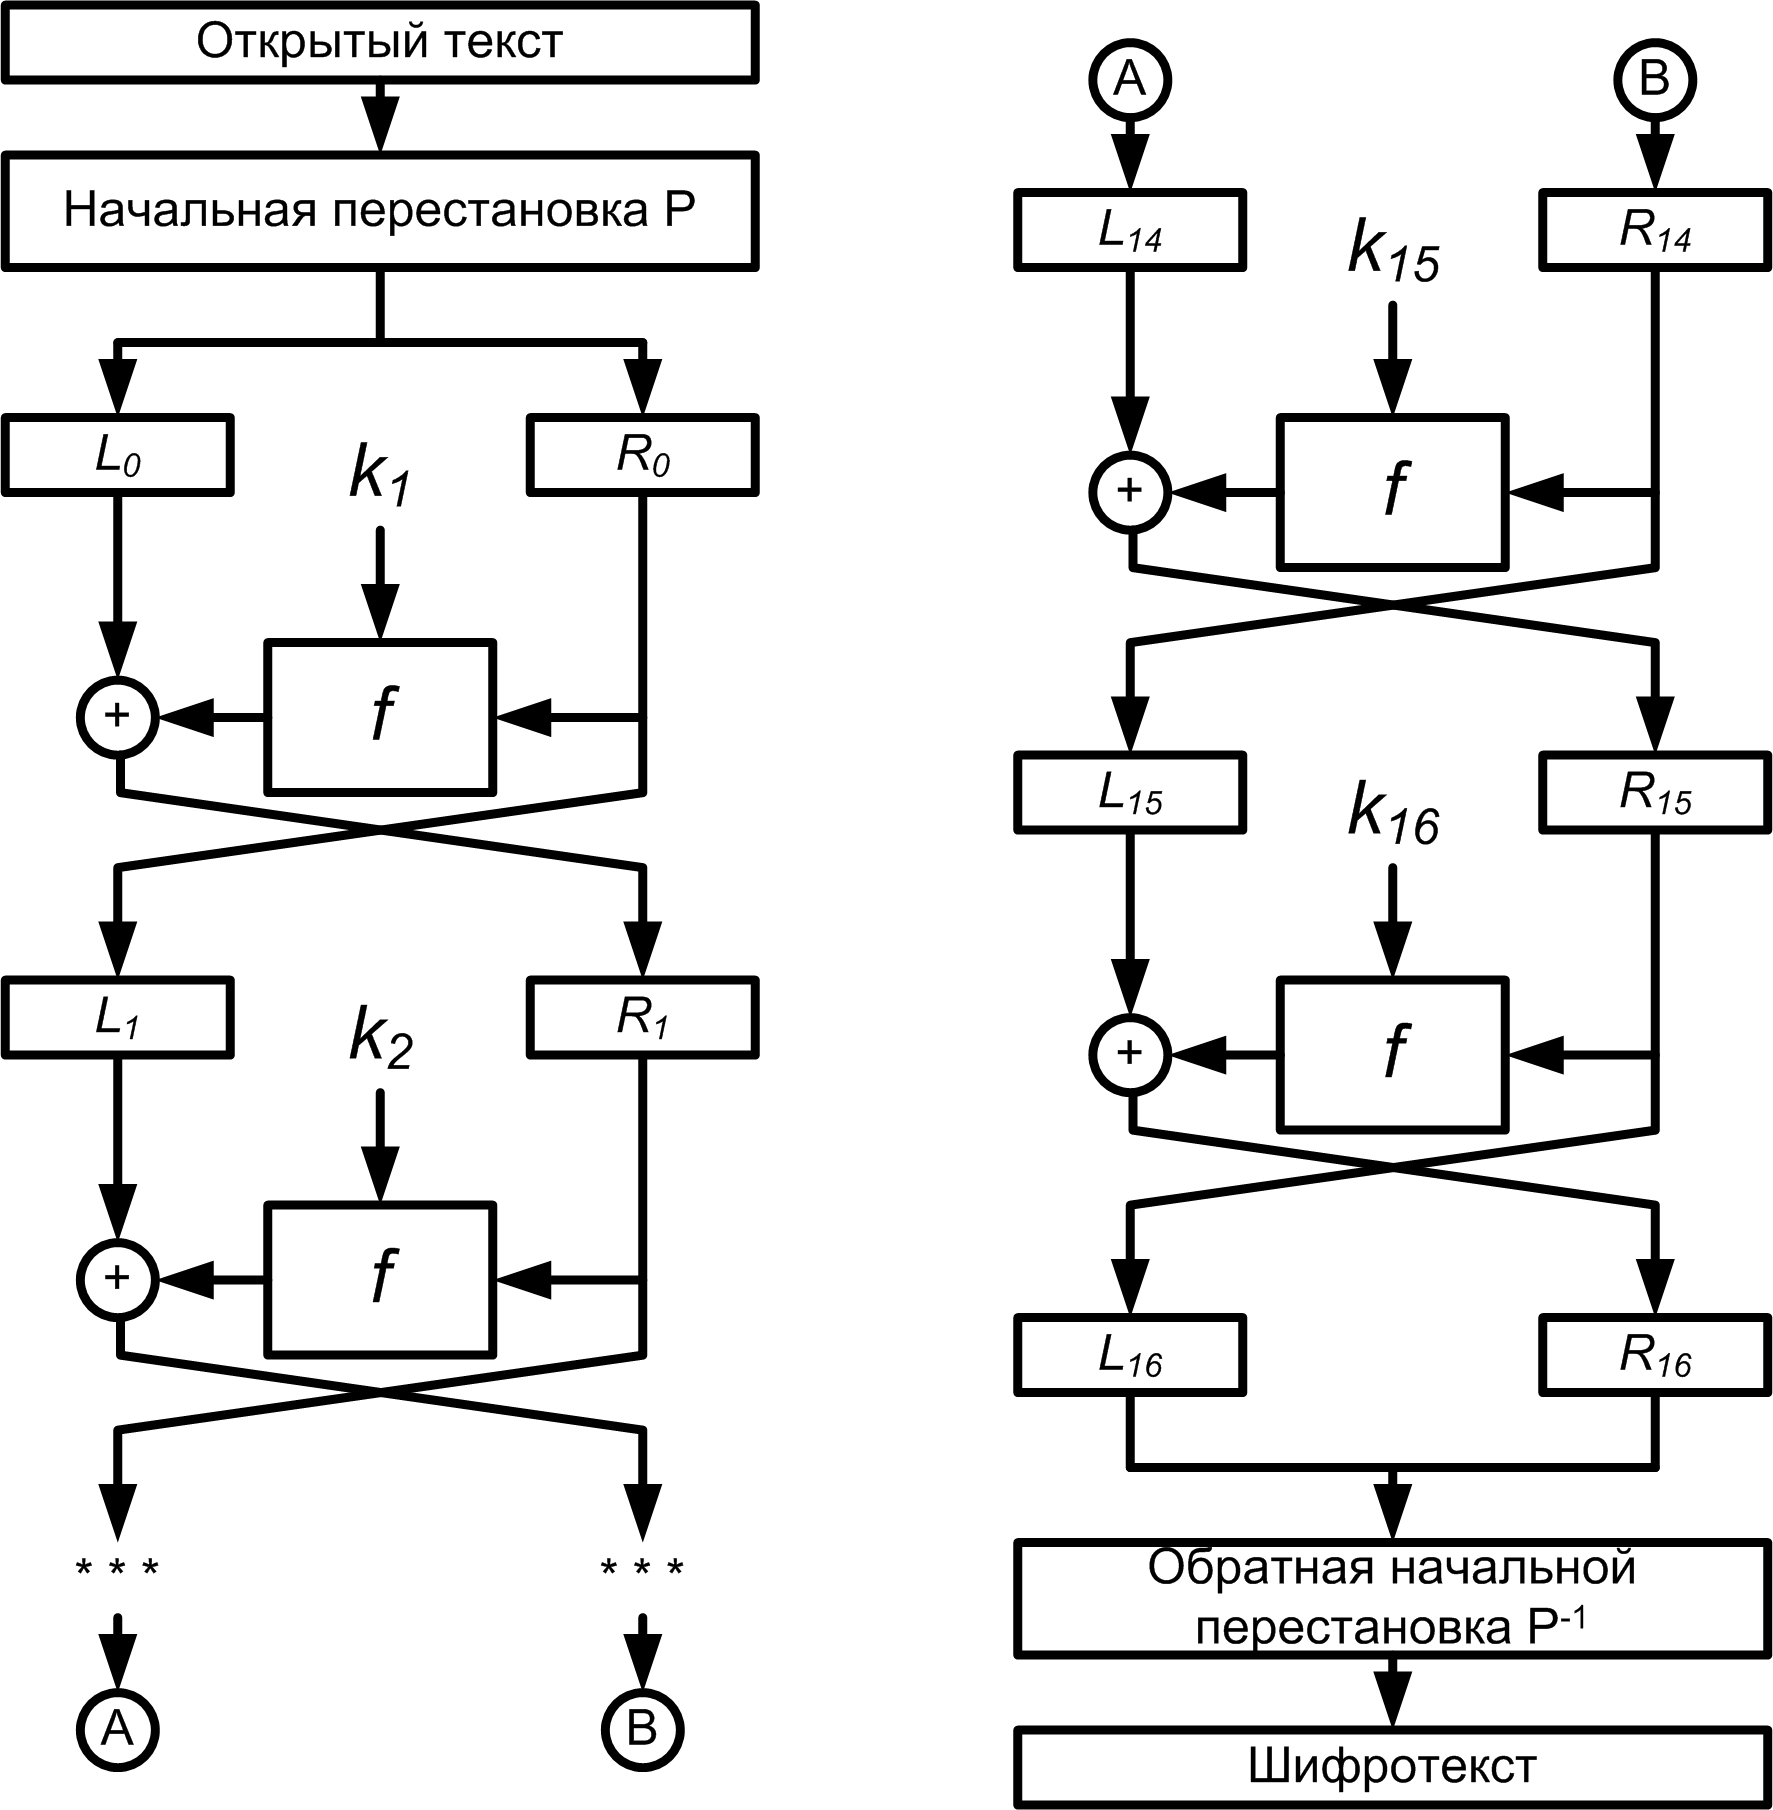
\includegraphics[height=.74\textheight]{pict/desrounds} }
            \mode<article>{ 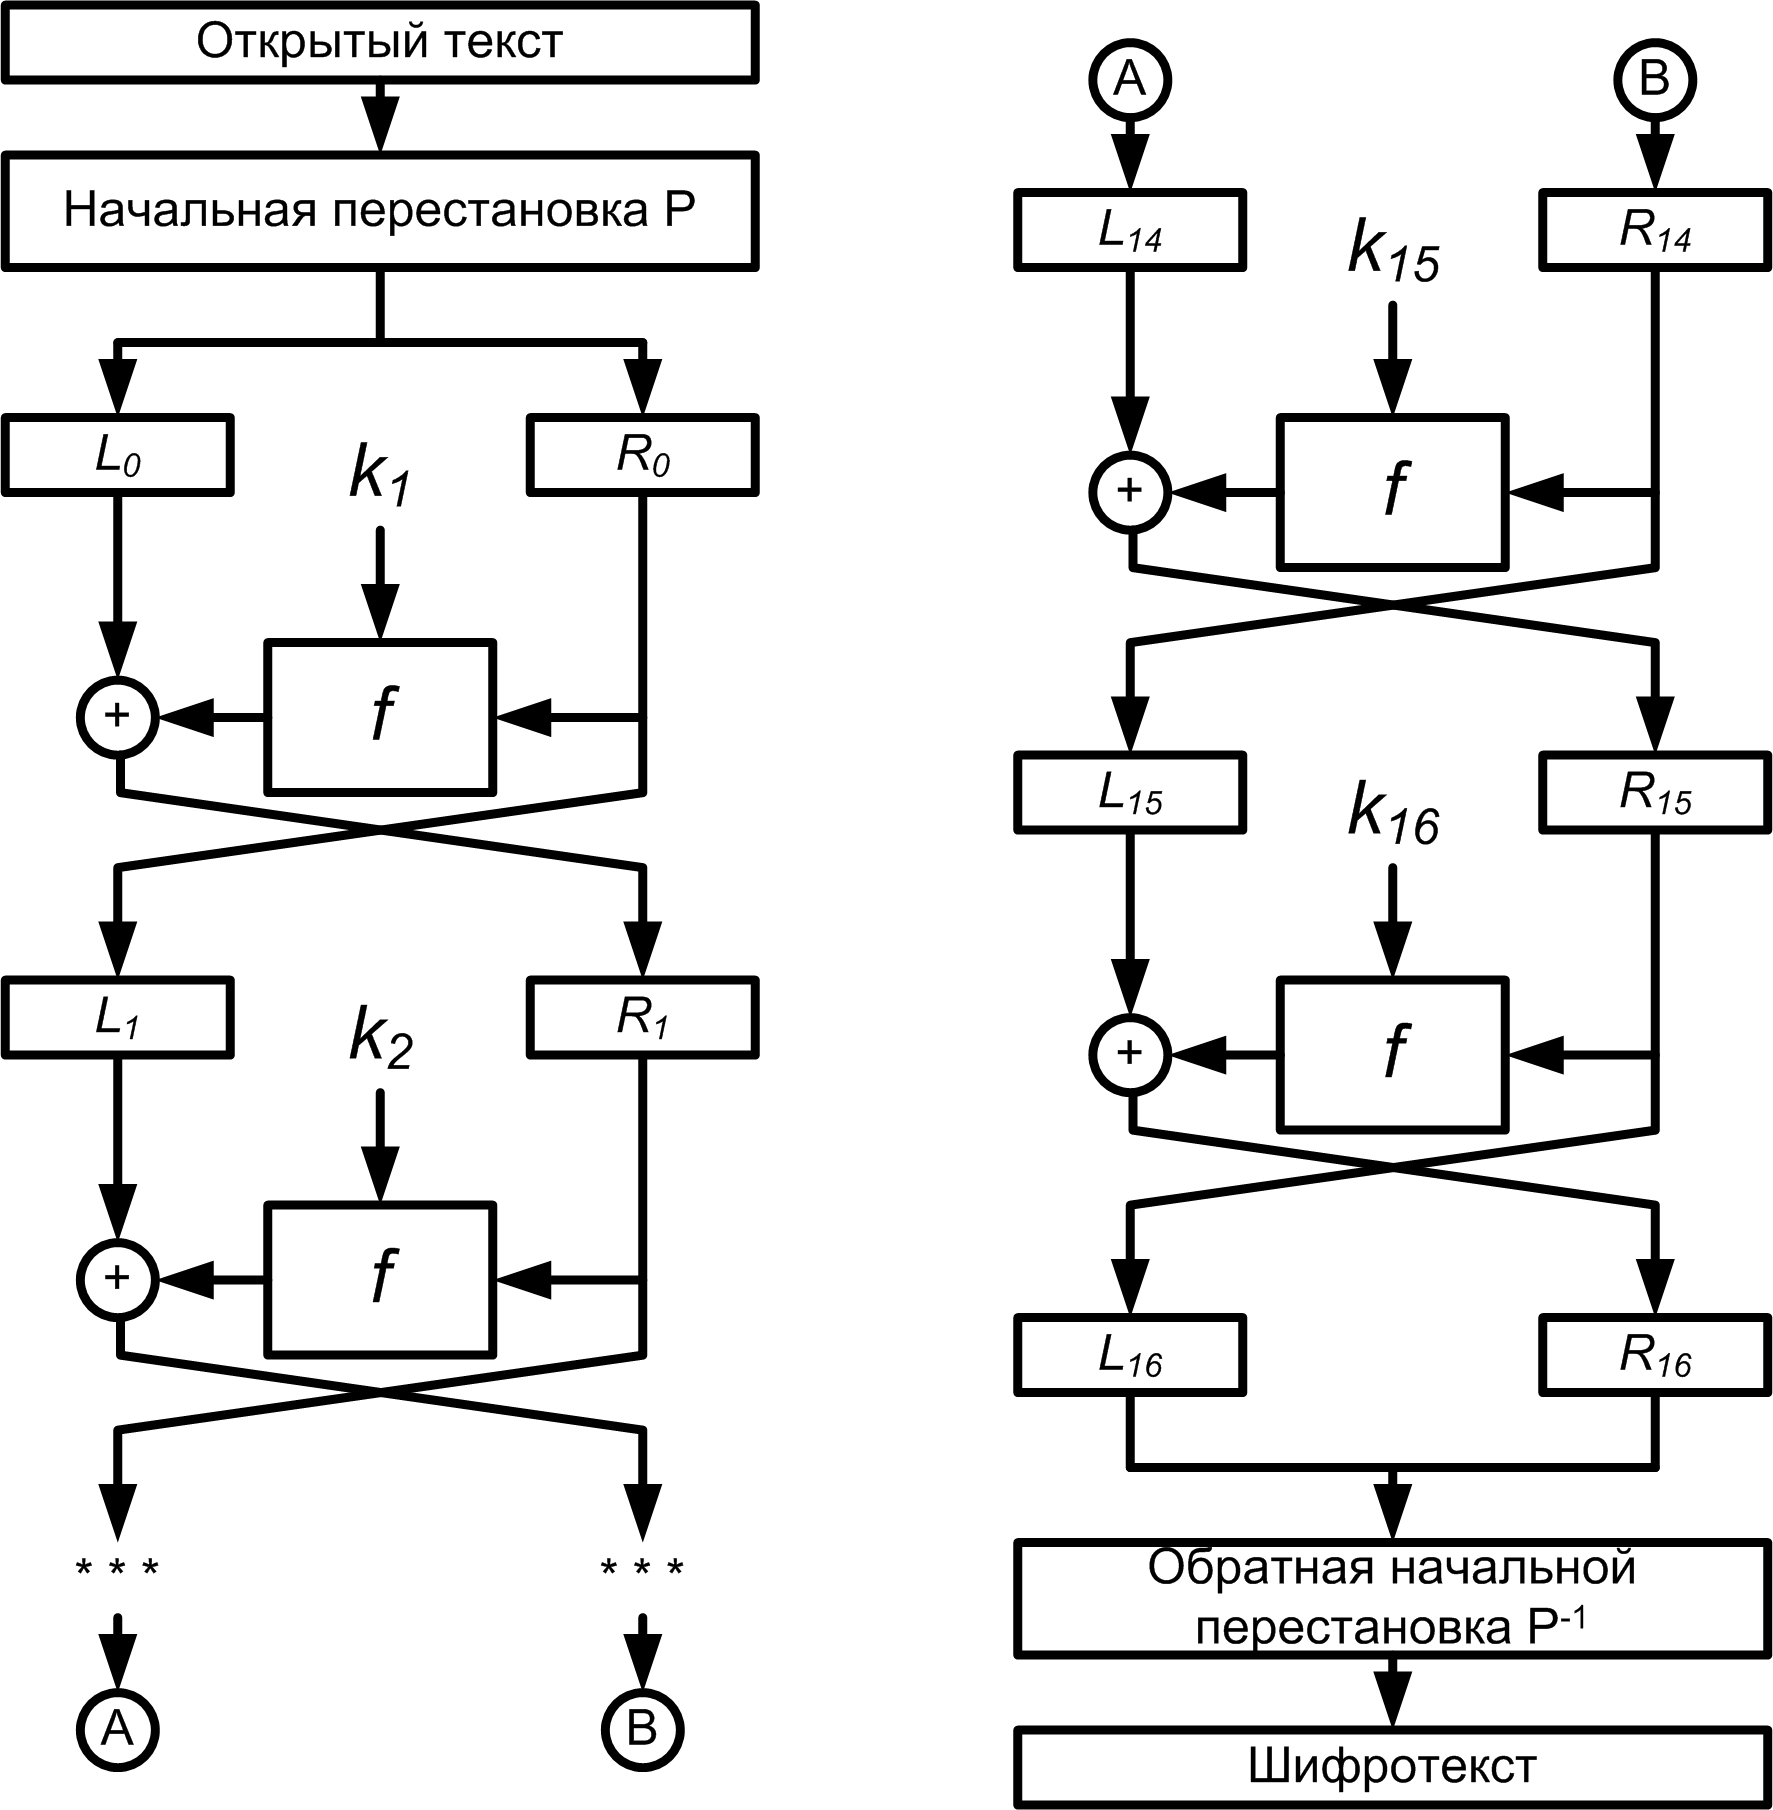
\includegraphics[width=.74\textwidth]{pict/desrounds} }
        \end{center}
        \caption{Блок Фейстеля для DES}\label{pict:desrounds}
    \end{figure}
    \mode<article>{См. рисунок \ref{pict:desrounds}}
\end{frame}


Интерес представляет структура используемого преобразования $f$:


\begin{frame}
    \frametitle{Блок Фейстеля для DES}

    \begin{figure}
        \begin{center}
            \mode<presentation>{ 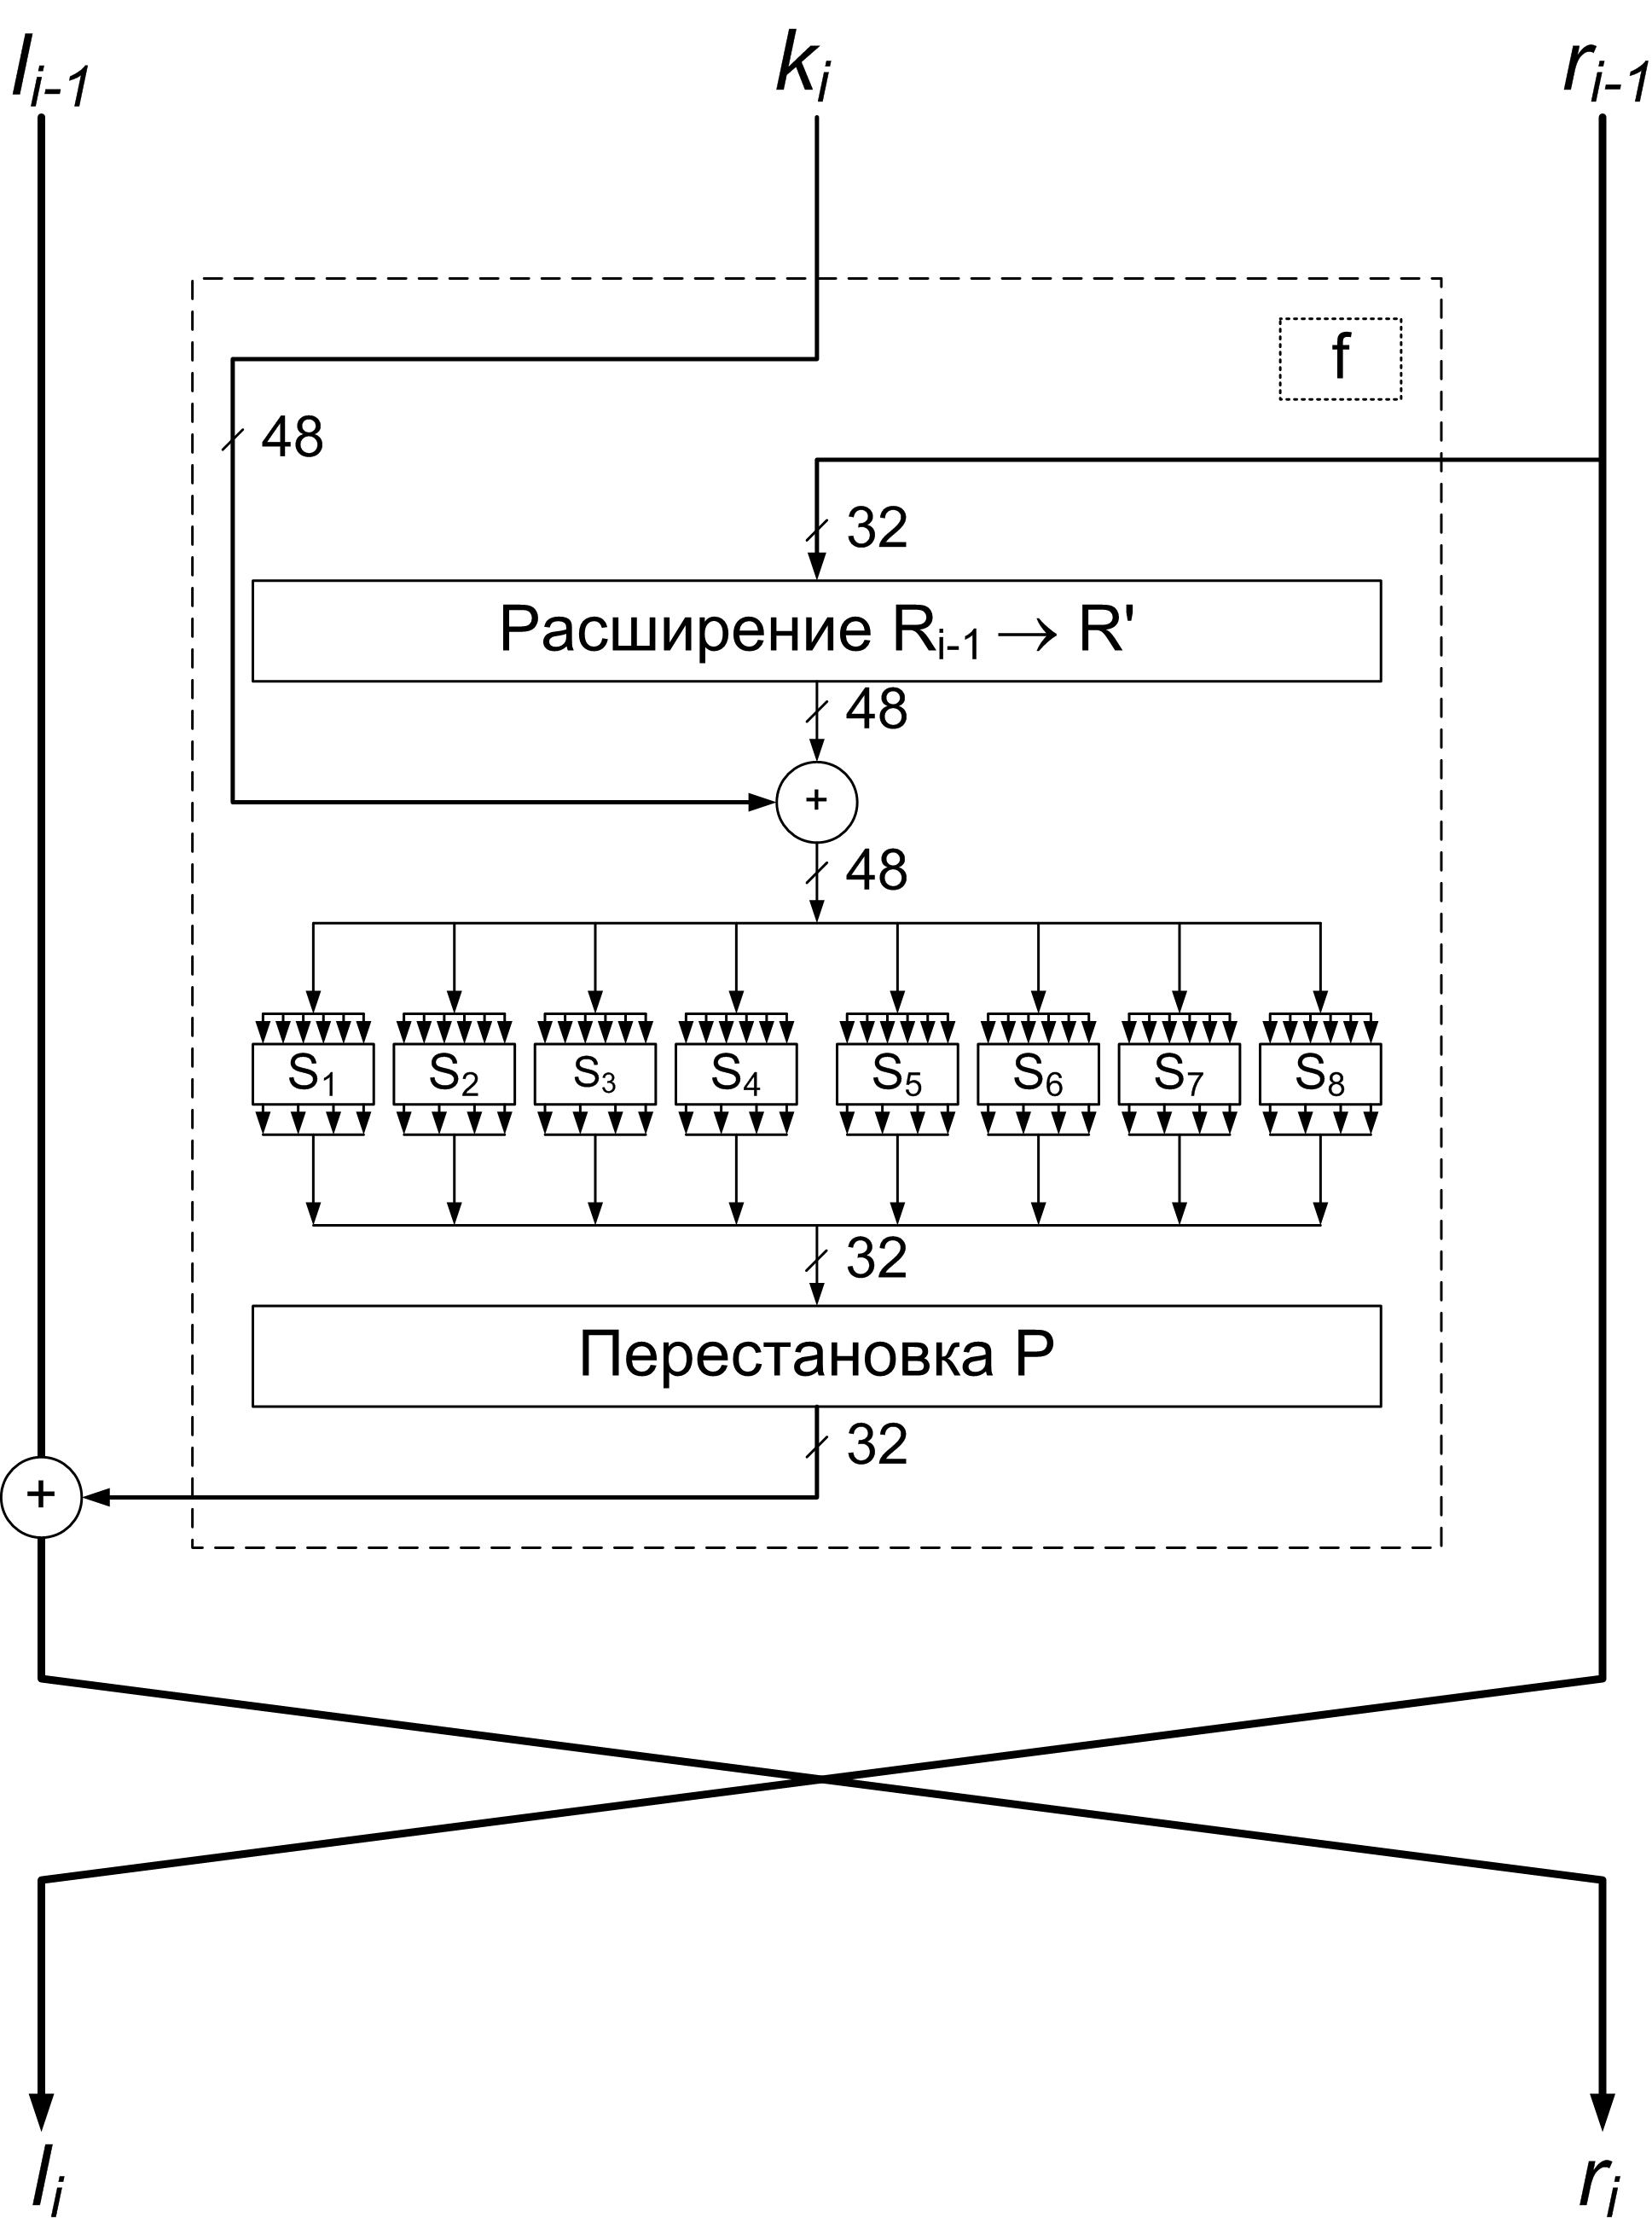
\includegraphics[height=.74\textheight]{pict/des} }
            \mode<article>{ 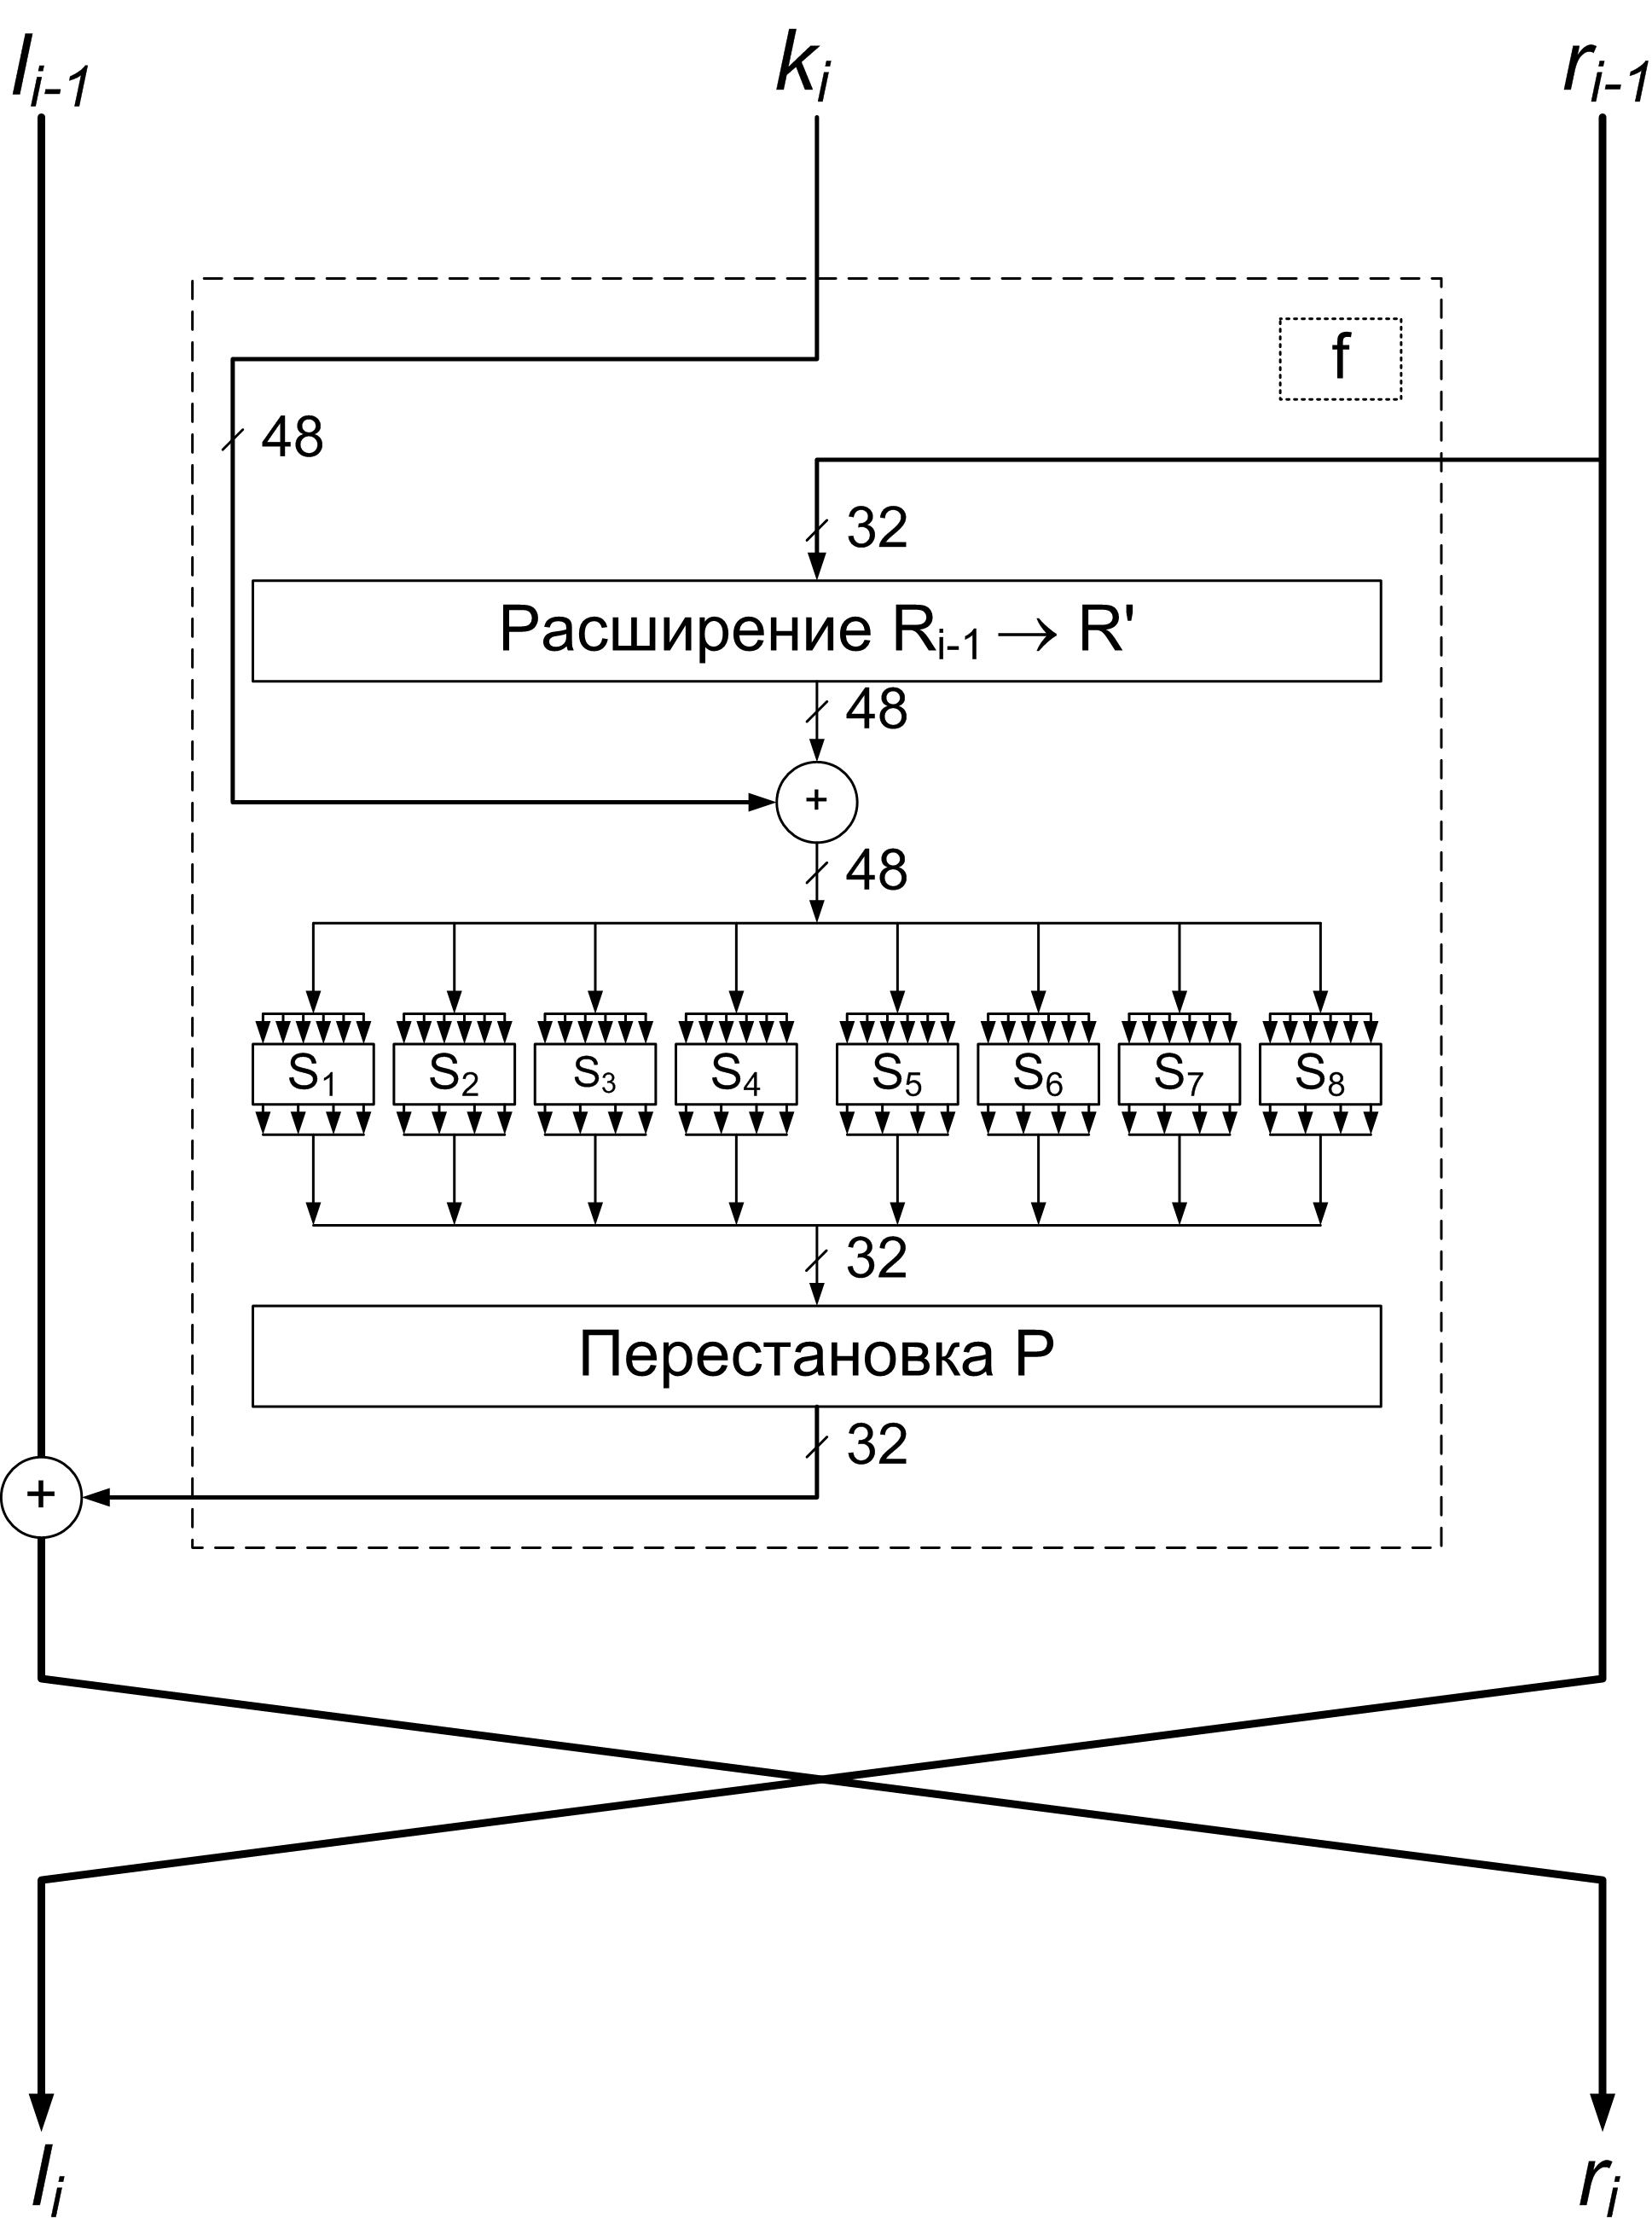
\includegraphics[width=.74\textwidth]{pict/des} }
        \end{center}
        \caption{Блок Фейстеля для DES}\label{pict:des}
    \end{figure}
    \mode<article>{См. рисунок \ref{pict:des}}
\end{frame}

Поступающая на вход 32-х битная <<правая>> ($r_{i-1}$) половинка исходных данных подвергается расширению до 48 бит:

\begin{frame}
    \frametitle{Расширение}

    \begin{figure}
        \begin{center}
            \mode<presentation>{ 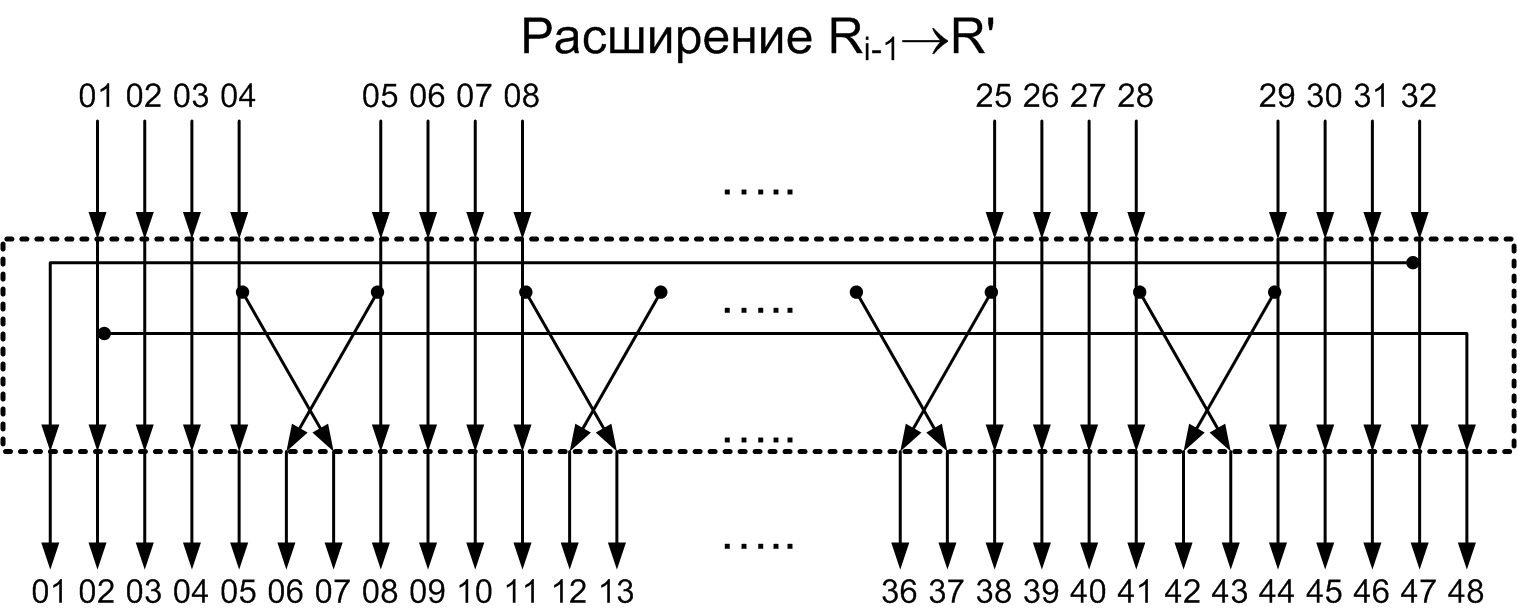
\includegraphics[width=.94\textwidth]{pict/desR} }
            \mode<article>{ 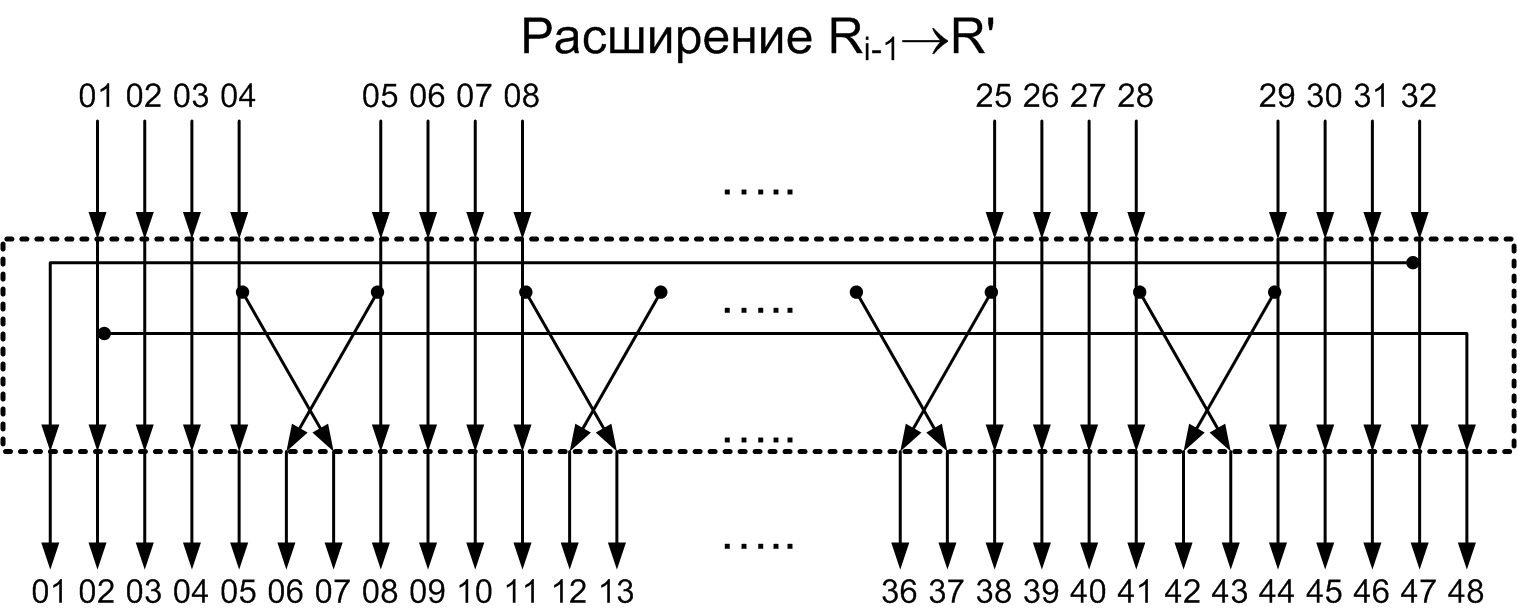
\includegraphics[width=.74\textwidth]{pict/desR} }
        \end{center}
        \caption{Расширяющий блок}\label{pict:desR}
    \end{figure}
    \mode<article>{См. рисунок \ref{pict:desR}}
\end{frame}

И по <<исключающему или>> побитно складывается с 48-битным ключом. Результат разбивается на 8 шестибитных подблоков. Каждый подблок поступает на $S$ блок, осуществляющий подстановку $6\times 4$ и дающий на выходе 4 бита. На рисунке приведена таблица подстановки для блока $S_1$ (все подстановки $S_1\ldots S_8$ различны!). Исходные 6 бит разбиваются на две группы $\langle v_1, v_2\rangle$ по 2 и 4 бита соответственно. Число $v_1$ --- индекс строки, а $v_2$ --- столбца.

\begin{frame}
    \frametitle{Подстановка $S_1\in\{S_1,\ldots,S_8\}$.}

    \[
        S_1 =
        \left(
            \begin{array}[c]{c@{\ }c@{\ }c@{\ }c@{\ }c@{\ }c@{\ }c@{\ }c@{\ }c@{\ }c@{\ }c@{\ }c@{\ }c@{\ }c@{\ }c@{\ }c@{\ }}
                14  &4   &13  &1   &2   &15  &11  &8   &3   &10  &6   &12  &5   &9   &0   &7 \\
                0   &15  &7   &4   &14  &2   &13  &1   &10  &6   &12  &11  &9   &5   &3   &8 \\
                4   &1   &14  &8   &13  &6   &2   &11  &15  &12  &9   &7   &3   &10  &5   &0 \\
                15  &12  &8   &2   &4   &9   &1   &7   &5   &11  &3   &14  &10  &0   &6   &13
            \end{array}
        \right)
    \]
\end{frame}

Получившиеся в результате 8 4-х битных подблоков объединяются в один 32-битный блок и поступают на блок перестановки:

\begin{frame}
    \frametitle{Перестановка $P$}

    \[
        P =
        \left(
            \begin{array}[c]{c@{\ }c@{\ }c@{\ }c@{\ }c@{\ }c@{\ }c@{\ }c@{\ }c@{\ }c@{\ }c@{\ }c@{\ }c@{\ }c@{\ }c@{\ }c@{\ }}
                16  &7  &20 &21 &29 &12 &28 &17 &1  &15 &23 &26 &5  &18 &31 &10 \\
                2   &8  &24 &14 &32 &27 &3  &9  &19 &13 &30 &6  &22 &11 &4  &25 \\
            \end{array}
        \right)
    \]
\end{frame}

Результат перестановки складывается по модулю 2 побитно с левой половинкой исходных данных раунда. Получившийся 32-битный блок есть правая половинка выхода раунда, левая половинка на выходе есть правая половинка исходных данных раунда. 

В настоящее время длина ключа в 56 бит не является актуальной. Используют, например, 3DES, который формируется так (увеличивая тем самым длину ключа до 56*3=168 бит):


\begin{frame}
    \frametitle{DES3, Tripple DES}

    \begin{figure}
        \begin{center}
            \mode<presentation>{ 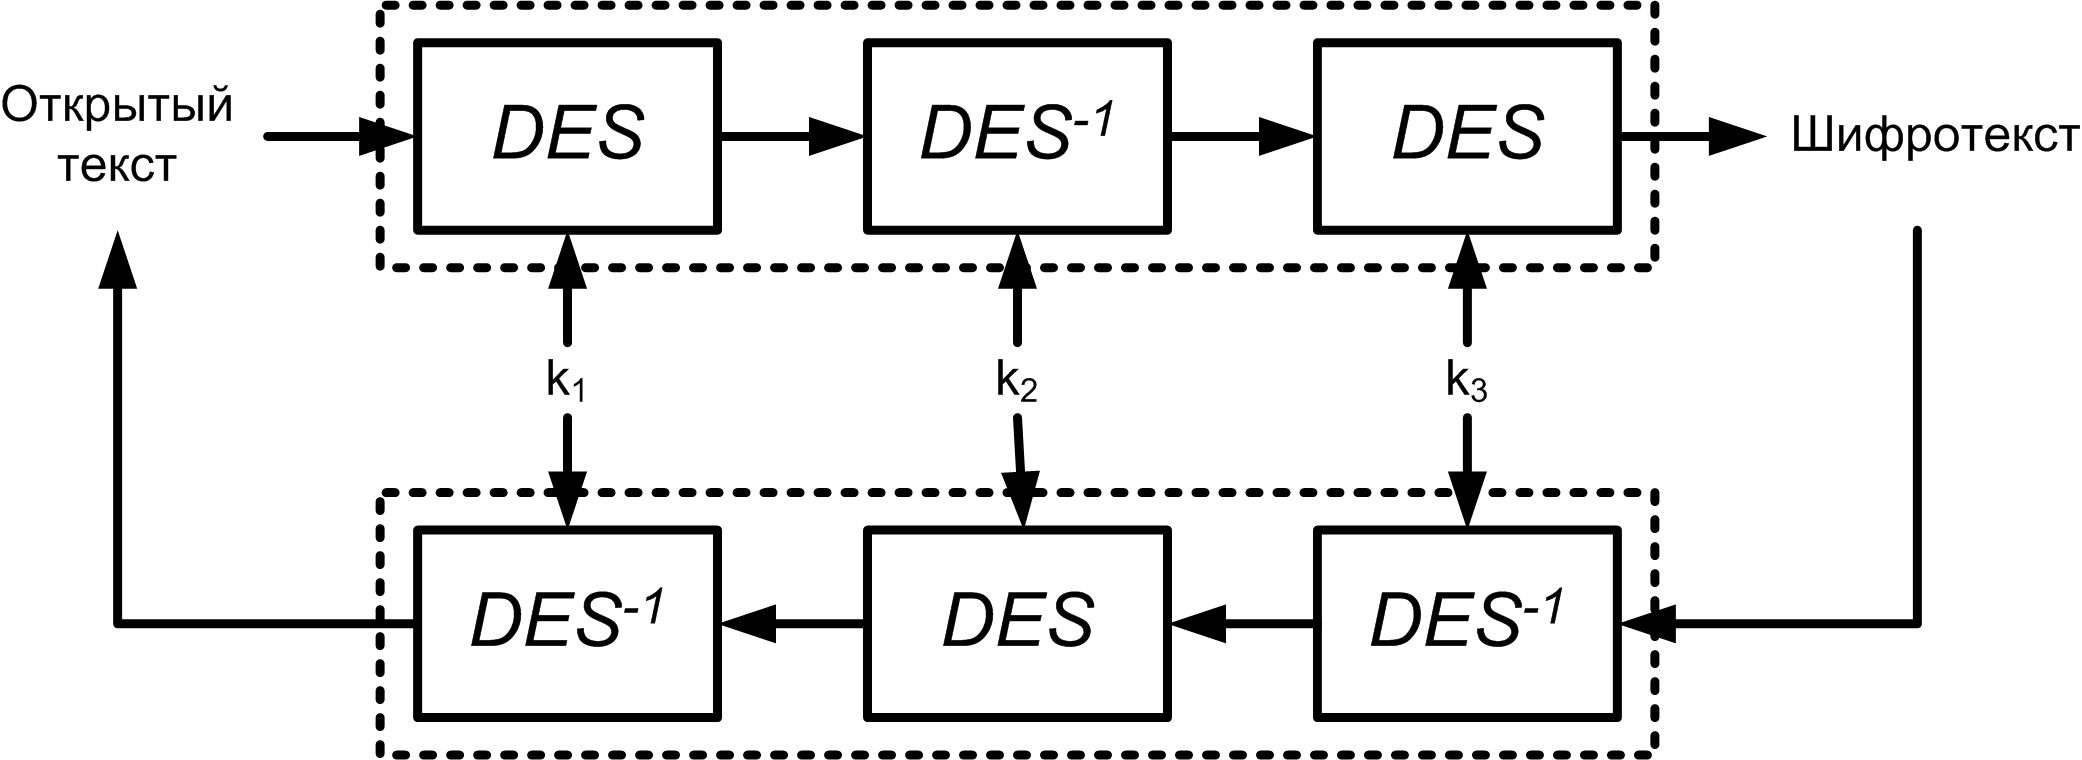
\includegraphics[width=.74\textwidth]{pict/des3} }
            \mode<article>{ 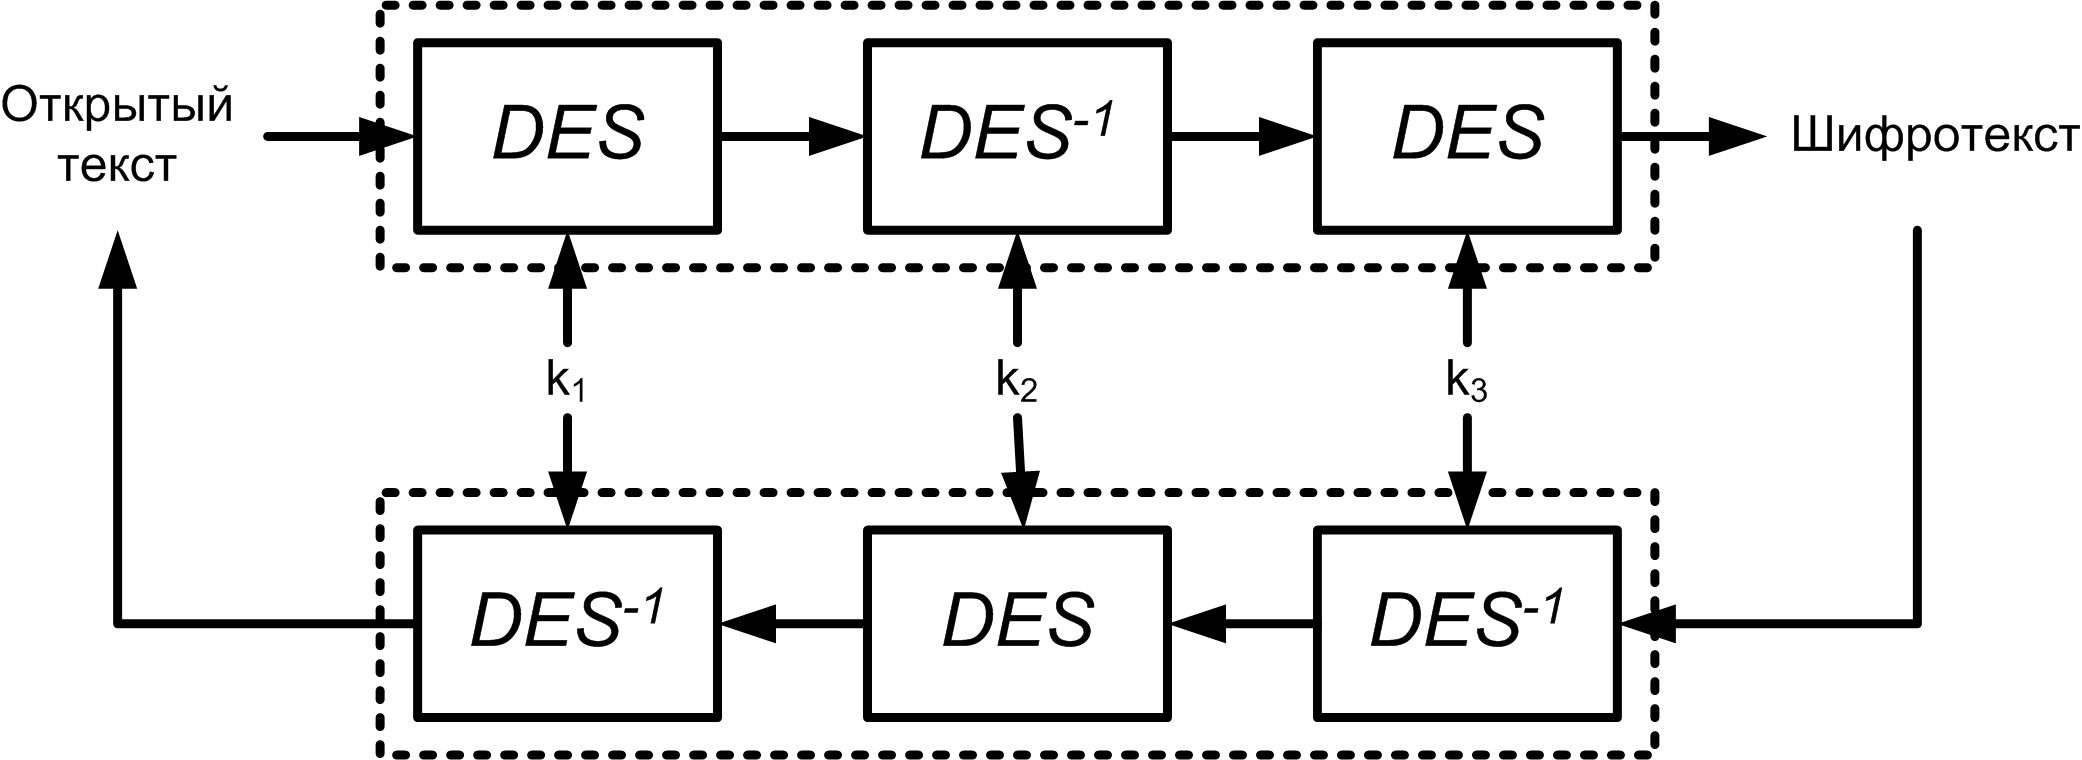
\includegraphics[width=.74\textwidth]{pict/des3} }
        \end{center}
        \caption{DES3}\label{pict:des3}
    \end{figure}
    \mode<article>{См. рисунок \ref{pict:des3}}
\end{frame}


\subsection{AES (Rijndael)}


\begin{frame}
    \frametitle{AES (Rijndael)}
    
    AES --- Advanced Encryption Standard. 2 октября 2000 года это почетное место занял шифр Rijndael, разработанный бельгийскими криптографами: Даменом (Daemen) и Рийменом (Rijmen).
    
    Размеры ключа и блоков этого шифра могут независимо друг от друга иметь размер в 128, 192 и 256 бит.
\end{frame}


\begin{frame}[fragile]
    \frametitle{AES (Rijndael)}
    \framesubtitle{Алгоритм}
    
    \begin{columns}
        \column{.49\textwidth}
            \begin{block}{Шифрование}
\begin{semiverbatim}
AddRoundKey(S,K[0])
for (i=1; i<=9; ++i) \{
    SubBytes(S);
    ShiftRows(S);
    MixColumns(S);
    AddRoundKey(S, K[i]);
\}
SubBytes(S);
ShiftRows(S);
AddRoundKey(S, K[10]);                
\end{semiverbatim}            
            \end{block}
        
        \column{.49\textwidth}
            \begin{block}{Расшифрование}
\begin{semiverbatim}
AddRoundKey(S, K[10]);                
InvShiftRows(S);
InvSubBytes(S);
for (i=9; i<=1; -{-}i) \{
    AddRoundKey(S, K[i]);
    InvMixColumns(S);
    InvShiftRows(S);
    InvSubBytes(S);
\}
AddRoundKey(S,K[0])
\end{semiverbatim}            
            \end{block}
    \end{columns}
\end{frame}


\begin{frame}
    \frametitle{AES (Rijndael)}
    
    Рассмотрим шифр при размере блока 128 бит и размере ключа 128 бит. При этом 128-битный блок $b$ рассматривается как матрица байт\footnote{Байт = 8 Бит.}, размером $4\times 4$.
    \[
        b=
        \begin{pmatrix}
            b_0 & b_4 & b_8     & b_{12} \\
            b_1 & b_5 & b_9     & b_{13} \\
            b_2 & b_6 & b_{10}  & b_{14} \\
            b_3 & b_7 & b_{11}  & b_{15}
        \end{pmatrix},
    \]
    где $b_i$ --- байты блока. 
    
    На основе ключа генерируется еще 10 подключей для раундов шифрования \footnote{Не будем заострять внимание на этой процедуре, называемой процедурой \alert{разворачивания ключа}}.
\end{frame}


\begin{frame}
    \frametitle{AES (Rijndael)}
    \framesubtitle{SubBytes($S$)}
    
    \begin{enumerate}
        \item Для каждого байта $x$ матрицы $S$ находится обратный элемент $x^{-1}$ в поле $F_{2^8}[X]/(X^8+X^4+X^3+X+1)$. Для $x=0$ по соглашению $x^{-1}=0$
        \item Далее $x^{-1}$ рассматривается как 8-разрядный вектор и находится линейное преобразование в поле $F_2$:
        \[
            y=
            \begin{pmatrix}
                1&0&0&0&1&1&1&1\\
                1&1&0&0&0&1&1&1\\
                1&1&1&0&0&0&1&1\\
                1&1&1&1&0&0&0&1\\
                1&1&1&1&1&0&0&0\\
                0&1&1&1&1&1&0&0\\
                0&0&1&1&1&1&1&0\\
                0&0&0&1&1&1&1&1\\
            \end{pmatrix}\cdot x^{-1} + 
            \begin{pmatrix}
                1\\
                1\\
                0\\
                0\\
                0\\
                1\\
                1\\
                0
            \end{pmatrix}
        \]
    \end{enumerate}
    Имеется обратное преобразование InvSubBytes($S$).
\end{frame}


\begin{frame}
    \frametitle{AES (Rijndael)}
    \framesubtitle{ShiftRows($S$)}
    
    \[
        \begin{pmatrix}
            \fbox{$s_{0,0}$}    & s_{0,1}           & s_{0,2}           &  \fbox{$s_{0,3}$} \\ 
            s_{1,0}             & \fbox{$s_{1,1}$}  & s_{1,2}           &  \fbox{$s_{1,3}$} \\ 
            s_{2,0}             & s_{2,1}           & \fbox{$s_{2,2}$}  &  \fbox{$s_{2,3}$} \\ 
            s_{3,0}             & s_{3,1}           & s_{3,2}           &  \fbox{$s_{3,3}$}
        \end{pmatrix}
        \to
        \begin{pmatrix}
            \fbox{$s_{0,0}$}    & s_{0,1}           & s_{0,2}           &  \fbox{$s_{0,3}$} \\ 
            \fbox{$s_{1,1}$}    & s_{1,2}           &  \fbox{$s_{1,3}$} & s_{1,0}\\ 
            \fbox{$s_{2,2}$}    &  \fbox{$s_{2,3}$} & s_{2,0}           & s_{2,1}\\ 
            \fbox{$s_{3,3}$}    & s_{3,0}           & s_{3,1}           & s_{3,2}
        \end{pmatrix}
    \]
    Имеется обратное преобразование InvShiftRows($S$).
\end{frame}


\begin{frame}
    \frametitle{AES (Rijndael)}
    \framesubtitle{MixColumns($S$)}
    
    $j$-й столбец интерпретируется как полином 
    \[
        b_j(X) = s_{3,j}X^3 + s_{2,j}X^2 + s_{1,j}X + s_{0,j},
    \]
    где байт $s_{i,j}\in F_{2^8}[X]/(X^8+X^4+X^3+X+1)$.
    
    Результат преобразования столбца получается так:
    \[
        b_j(X)'\equiv c(X)\cdot b_j(X)\pmod{\fbox{0x01}X^4+\fbox{0x01}},
    \]
    где $c(X)=\fbox{0x03}X^3 + \fbox{0x01}X^2 + \fbox{0x01}X + \fbox{0x02}$.
    
    Имеется обратное преобразование InvMixColumns($S$).
\end{frame}


\begin{frame}
    \frametitle{AES (Rijndael)}
    \framesubtitle{AddRoundKey($S$, $K$)}

    Для каждого байта матрицы $S$ выполняется побитное сложение в $F_2$ с соответствующим байтом ключа $K$.
    \[s_{i,j}'=s_{i,j}\oplus k_{i,j}.\]
    
    Обратное преобразование, очевидно, и есть AddRoundKey($S$, $K$).
\end{frame}


\begin{frame}
    \frametitle{AES (Rijndael)}
    \framesubtitle{Заключение}

    \begin{itemize}
        \item Имеет быстродейтсвющую и стойкую реализацию\footnote{В частности, благодаря табличной реализации операций над полями, время выполнения не зависит от операндов, что исключает тайминг-атаки (временной анализ) на шифр.}
        \item Математически обоснован.
        \item Не использует блоки Файстеля, шифрование и дешифрование требуют применения различных программ или аппаратных схем.
    \end{itemize}
\end{frame}


\section{Асимметричные схемы}


\subsection{RSA}

    
\begin{frame}
    \frametitle{RSA}

    \begin{table}[ht]
        \centering
        \mode<article>{\caption{RSA}\label{t:rsacipher}}
        \begin{tabular}[c]{p{0.25\textwidth}|p{0.65\textwidth}}
            \hline\hline
            Открытый ключ & $\langle n,e\rangle$. $n=pq$ --- произведение \alert{простых} чисел $p$ и $q$ (которые хранятся в \alert{секрете}), $e$ --- произвольно выбираемое число, взаимно простое с $\phi(n)=(p-1)(q-1)$ \\ \hline
            Секретный ключ & $d\equiv e^{-1}\pmod{\phi(n)}$\\ \hline
            Шифрование & $c\equiv m^e\pmod{n}$\\ \hline
            Расшифрование & $m\equiv c^d\equiv {(m^e)}^d\equiv m^{ed}\equiv m^{k\phi(n)+1}\equiv m\cdot m^{k\phi(n)}\equiv m\cdot 1 \pmod{n}$\\ 
            \hline\hline
        \end{tabular}
    \end{table}
    \mode<article>{см. табл. \ref{t:rsacipher}.}
\end{frame}


\subsection{Криптосистема ЭльГамаля}


\begin{frame}
    \frametitle{Криптосистема ЭльГамаля}
    \framesubtitle{Шифрование}

    \begin{table}[ht]
        \centering
        \mode<article>{\caption{Криптосистема ЭльГамаля. Шифрование}\label{t:ElGamalCipher}}
        \begin{tabular}[c]{p{0.35\textwidth}|p{0.55\textwidth}}
            \hline\hline
            Открытый ключ & $\langle p,g,y\rangle$. $p$ --- простое число. $g<p$. $y\equiv g^x\pmod{p}$ \\ \hline
            Секретный ключ & $x<p$\\ \hline
            Шифрование & $k$ выбирается случайным образом, взаимно простое с $\phi(p)=p-1$\\ 
            1-я часть шифротекста & $a\equiv g^k\pmod{p}$\\
            2-я часть шифротекста & $b\equiv M\cdot y^k\pmod{p}$\\ \hline
            Расшифрование & $M \equiv \frac{b}{a^x} \equiv \frac{M\cdot g^{xk}}{g^{kx}}\pmod{p}$\\
            \hline\hline
        \end{tabular}
    \end{table}
    \mode<article>{см. табл. \ref{t:ElGamalCipher}.}
\end{frame}


\begin{frame}
    \frametitle{Криптосистема ЭльГамаля}
    \framesubtitle{Цифровая подпись}

    \begin{table}[ht]
        \centering
        \mode<article>{\caption{Криптосистема ЭльГамаля. Цифровая подпись}\label{t:ElGamalSign}}
        \begin{tabular}[c]{p{0.25\textwidth}|p{0.65\textwidth}}
            \hline\hline
            Открытый ключ       & $\langle p,g,y\rangle$. $p$ --- простое число. $g<p$.\\
                                & $y\equiv g^x\pmod{p}$ \\ \hline
            Секретный ключ      & $x<p$\\ \hline
            Получение ЦП        & $k$ выбирается случайным образом, взаимно простое с $\phi(p)=p-1$\\ 
            1-я часть подписи   & $a\equiv g^k\pmod{p}$\\
            2-я часть подписи   & $b$ такое, что $M\equiv(xa+kb)\pmod{p-1}$\\ \hline
            Проверка подписи    & Подпись верна, если $y^{a}a^{b}\equiv g^M\pmod{p}$\\
                                & $y^{a}a^{b} \equiv g^{xa}g^{kb} \equiv g^{xa+kb} \equiv g^{M}g^{(p-1)m} \pmod{p}$\\
            \hline\hline
        \end{tabular}
    \end{table}
    \mode<article>{см. табл. \ref{t:ElGamalSign}.}
\end{frame}


\subsection{Эллиптические кривые}


\begin{frame}
    \frametitle{Криптосистема ЭльГамаля в эллиптических кривых}
    \framesubtitle{Шифрование}

    \begin{table}[ht]
        \centering
        \mode<article>{\caption{Криптосистема ЭльГамаля в эллиптических кривых. Шифрование}\label{t:ElGamalElliCipher}}
        \begin{tabular}[c]{p{0.35\textwidth}|p{0.55\textwidth}}
            \hline\hline
            Открытый ключ & $\langle E,P,Y\rangle$. $E$ --- эллиптическая кривая. $P$ --- точка большого порядка на кривой $E$. $Y=kP$. \\ \hline
            Секретный ключ & $k\in\mathbb{Z}$\\ \hline
            Шифрование & Сообшение отображается\footnote{Делали этого процесса опущены} на точку кривой $M\in E$. Выбирается случайное $r\in\mathbb{Z}$.\\ 
            Шифротекст & $C=\langle C_1,C_2\rangle=\langle rP,M+rY\rangle$\\
            Расшифрование & $-kC_1+C_2=-krP+M+rY=-krP+M+rkP=M$\\
            \hline\hline
        \end{tabular}
    \end{table}
    \mode<article>{см. табл. \ref{t:ElGamalElliCipher}.}
\end{frame}


\begin{frame}
    \frametitle{Криптосистема ЭльГамаля в эллиптических кривых}
    \framesubtitle{Цифровая подпись. ECDSA}

    \begin{table}[ht]
        \centering
        \mode<article>{\caption{Криптосистема ЭльГамаля в эллиптических кривых. Цифровая подпись}\label{t:ElGamalElliSign}}
        \begin{tabular}[c]{p{0.25\textwidth}|p{0.65\textwidth}}
            \hline\hline
            Открытый ключ   & $\langle E,P,N,Y\rangle$. $E$ --- эллиптическая кривая. 
                              $P$ --- точка большого порядка $N$ на $E$. 
                              $Y=kP$. \\ \hline
            Секретный ключ  & $k\in\mathbb{Z}$\\ \hline
            Получение ЦП    & Выбирается случайное $r\in\mathbb{Z}$ такое, 
                              что для точки $R=rP=(x,y)$, координата $x\neq 0$. \\ 
            Подпись         & $\langle c,d\rangle$. Где $c,d\neq 0$ 
                              (иначе повторить выбор $r$). $c\equiv(x+H(M))\pmod{N}$. 
                              $d\equiv(r-ck)\pmod{N}$\\
            Проверка        & $R=dP+cY=dP+ckP=(x',y')$. Проверить $H(M')\equiv(c-x') \pmod{N}$\\
            \hline\hline
        \end{tabular}
    \end{table}
    \mode<article>{см. табл. \ref{t:ElGamalElliSign}.}
    Отечественный стандарт цифровой подписи ГОСТ Р 34.10-2001 также основан на эллиптической кривой.
\end{frame}


%TODO нужно нарыть о стандартах в криптографии, ITU (X.509), RFC, PKCS

\appendix


\begin{frame}
\frametitle{Источники и полезные ссылки}
\begin{enumerate}
    \item \alert{Источники}. 
    
    Основные схемы см. в \cite{bib:chmora:crypto,bib:shangin:protect,bib:shneir:applCrypto}. Математические основы см. в \cite{bib:mao:modernCrypto,bib:smart:crypto}. Подробнее об криптографии на эллиптических кривых см. в \cite{bib:bolotov:elliptic, bib:bolotov:ellipticProtocol}. Практические схемы рассматриваются в \cite{bib:mao:modernCrypto,bib:shneir:applCrypto,bib:smart:crypto,bib:shangin:protect}. Отдельных рекомендаций заслуживает ставшая классикой \cite{bib:shneir:applCrypto}.
\end{enumerate}    
\end{frame}

\begin{frame}[allowframebreaks]{Библиография}
    \bibliographystyle{gost780u}
    \bibliography{./../bibliobase}
\end{frame}

\end{document}